% Copyright 2004 by Till Tantau <tantau@users.sourceforge.net>.
%
% In principle, this file can be redistributed and/or modified under
% the terms of the GNU Public License, version 2.
%
% However, this file is supposed to be a template to be modified
% for your own needs. For this reason, if you use this file as a
% template and not specifically distribute it as part of a another
% package/program, I grant the extra permission to freely copy and
% modify this file as you see fit and even to delete this copyright
% notice. 

%\documentclass[13pt,handout]{beamer}
\documentclass[13pt]{beamer}

\title{Following the Leader and Fast Rates in Linear Prediction: Curved Constraint Sets and Other Regularities}
\author{Ruitong Huang$^1$ \and Tor Lattimore$^2$  \\ \medskip
\textbf{Andr\'as Gy\"orgy$^3$} \and
{Csaba Szepesv\'ari$^1$}}
%\\
%joint work with  and }
\institute{$^1$Department of Computing Science\\University of Alberta\\ \smallskip
$^2$ School of Informatics and Computing, Indiana University \\ \smallskip
$^3$Department of Electrical and Electronic Engineering\\ Imperial College London}
\date{\tiny Lille, November 28, 2016} % Lille



% If you have a file called "university-logo-filename.xxx", where xxx
% is a graphic format that can be processed by latex or pdflatex,
% resp., then you can add a logo as follows:

\titlegraphic{ 
%
\includegraphics[height=10mm]{logo} \hspace{5pt}
}

%\pgfdeclareimage[height=0.5cm]{university-logo}{logo}
%\logo{\pgfuseimage{university-logo}}

% There are many different themes available for Beamer. A comprehensive
% list with examples is given here:
% http://deic.uab.es/~iblanes/beamer_gallery/index_by_theme.html
% You can uncomment the themes below if you would like to use a different
% one:
%\usetheme{AnnArbor}
%\usetheme{Antibes}
%\usetheme{Bergen}
%\usetheme{Berkeley}
%\usetheme{Berlin}
\usetheme{Boadilla}
%\usetheme{boxes}
%\usetheme{CambridgeUS}
%\usetheme{Copenhagen}
%\usetheme{Darmstadt}
%\usetheme{default}
%\usetheme{Frankfurt}
%\usetheme{Goettingen}
%\usetheme{Hannover}
%\usetheme{Ilmenau}
%\usetheme{JuanLesPins}
%\usetheme{Luebeck}
%\usetheme{Madrid}
%\usetheme{Malmoe}
%\usetheme{Marburg}
%\usetheme{Montpellier}
%\usetheme{PaloAlto}
%\usetheme{Pittsburgh}
%\usetheme{Rochester}
%\usetheme{Singapore}
%\usetheme{Szeged}
%\usetheme{Warsaw}

%%%%%%% Author defined area %%%%%%%%%%%%

%%%%%%%%%%%%%% TODOs %%%%%%%%%%%%%%%%%%%%%%%%%%%%%
\usepackage{color}
%\usepackage[usenames,dvipsnames]{xcolor}


\setbeamerfont{frametitle}{size=\large}


\usepackage[absolute,overlay]{textpos}
%%%%
% note: beamer slides are 128mm by 96 mm
\newcommand{\putatUL}[4]{ % width xpos ypos WHAT; upper left corner is put at the said pos
\begin{textblock*}{#1}[0,0](#2,#3)
#4
 \end{textblock*}
}
\newcommand{\putatUR}[4]{ % width xpos ypos WHAT; upper right corner is put at the said pos
\begin{textblock*}{#1}[1,0](#2,#3)
#4
 \end{textblock*}
 }
\newcommand{\putatUM}[4]{ % width xpos ypos WHAT; upper right corner is put at the said pos
\begin{textblock*}{#1}[0.5,0](#2,#3)
#4
 \end{textblock*}
 }
\newcommand{\putatBR}[4]{ % width xpos ypos WHAT; bottom right corner is put at the said pos
\begin{textblock*}{#1}[1,1](#2,#3)
#4
 \end{textblock*}
}
\newcommand{\putatBL}[4]{ % width xpos ypos WHAT; bottom left corner is put at the said pos
\begin{textblock*}{#1}[0,1](#2,#3)
#4
 \end{textblock*}
}
\newcommand{\putatBM}[4]{ % width xpos ypos WHAT; bottom left corner is put at the said pos
\begin{textblock*}{#1}[0.5,1](#2,#3)
#4
 \end{textblock*}
}
 \newcommand{\putatMID}[4]{ % width xpos ypos WHAT; mid of image is put at the said pos
\begin{textblock*}{#1}[0.5,0.5](#2,#3)
#4
 \end{textblock*}
 }

\newcommand{\putat}[3]{\begin{picture}(0,0)(0,0)\put(#1,#2){#3}\end{picture}} % xrelpos yrelpos WHAT

\newcommand{\bcol}[1][t]{\begin{columns}[#1]} % optional argument: alignment (t,b,c)
\newcommand{\ecol}{\end{columns}}
\newcommand{\col}[1][0.5\textwidth]{\column{#1}} % argument: width of the column


%%%%%
\usepackage{tikz}
\usetikzlibrary{calc,shapes.callouts,shapes.arrows}

% Usage example:
% \arrowthis{There is}{Corot} a\speechthis{beautiful flower}{Van Gogh}\bubblethis{in}{Matisse}\pointthis{the garden}{Monet}.        
%
% From: http://tex.stackexchange.com/questions/38805/simple-speech-bubbles-arrows-or-balloon-like-shapes-in-beamer        

\newcommand{\arrowthis}[2]{
        \tikz[remember picture,baseline]{\node[anchor=base,inner sep=0,outer sep=0]%
        (#1) {{#1}};
        \node[overlay,single arrow,draw=none,fill=red!50,anchor=tip,rotate=60] 
        at (#1.south) {#2};}%
    }%

\newcommand{\speechthis}[2]{
        \tikz[remember picture,baseline]{\node[anchor=base,inner sep=0,outer sep=0]%
        (#1) {{#1}};\node[overlay,ellipse callout,fill=blue!50] 
        at ($(#1.north)+(-.5cm,0.8cm)$) {#2};}%
    }%

\newcommand{\bubblethis}[2]{
        \tikz[remember picture,baseline]{\node[anchor=base,inner sep=0,outer sep=0]%
        (#1) {{#1}};\node[overlay,cloud callout,callout relative pointer={(-0.6cm,-0.7cm)},%
        aspect=2.5,fill=yellow!90] at ($(#1.north)+(2.5cm,1.6cm)$) {#2};}%
    }%

\newcommand{\pointthis}[2]{
        \tikz[remember picture,baseline]{\node[anchor=base,inner sep=0,outer sep=0]%
        (#1) {{#1}};\node[overlay,rectangle callout,%
        callout relative pointer={(0.2cm,0.7cm)},fill=green!50] at ($(#1.north)+(-.5cm,-1.4cm)$) {#2};}%
        }%
        
\newcommand{\leftpointthis}[2]{
        \tikz[remember picture,baseline]{\node[anchor=base,inner sep=0,outer sep=0]%
        (#1) {{#1}};\node[overlay,rectangle callout,%
        callout relative pointer={(0.2cm,0.7cm)},fill=green!50] at ($(#1.north)+(-.5cm,-1.4cm)$) {#2};}%
        }%

\newcommand{\rightpointthis}[2]{
        \tikz[remember picture,baseline]{\node[anchor=base,inner sep=0,outer sep=0]%
        (#1) {{#1}};\node[overlay,rectangle callout,%
        callout relative pointer={(-0.3cm,0.7cm)},fill=green] at ($(#1.north)+(.5cm,-1.4cm)$) {#2};}%
        }%        
%%%%%%%        

\renewcommand<>{\cancel}[1]{\alt#2{\beameroriginal{\cancel}{#1}}{#1}}


\setbeamertemplate{navigation symbols}{}
\setbeamertemplate{footline}[frame number]
\setbeamercolor{math text}{fg=blue!50!normal text.fg}

\usepackage{multimedia}


% uncomment the following line and comment the line after it if you want to turn
% off todos
%\usepackage[textwidth=\marginparwidth]{todonotes}
\usepackage[disable,backgroundcolor = White,textwidth=\marginparwidth]{todonotes}
\newcommand{\todoc}[2][]{\todo[color=Apricot!20,size=\tiny,#1]{#2}}
\newcommand{\todot}[2][]{\todo[color=Cerulean!20,size=\tiny,#1]{#2}}
\newcommand{\todoa}[2][]{\todo[color=Purple!20,size=\tiny,#1]{#2}}
\newcommand{\todor}[2][]{\todo[color=Blue!10,size=\tiny,#1]{#2}}

\usepackage{xspace}
\usepackage{mathtools}
\usepackage{graphicx}
\usepackage[round]{natbib}
\usepackage{xspace}
\usepackage{multicol}
\newcommand\Fontvi{\fontsize{6}{7.2}\selectfont}

\usepackage{esvect}

\allowdisplaybreaks
\newcommand{\cA}{\mathcal{A}}
\newcommand{\cB}{\mathcal{B}}
\newcommand{\cG}{\mathcal{G}}
\newcommand{\cX}{\mathcal{X}}
\newcommand{\cY}{\mathcal{Y}}
\newcommand{\cZ}{\mathcal{Z}}
\newcommand{\cW}{\mathcal{W}}
\newcommand{\cH}{\mathcal{H}}
\newcommand{\cF}{\mathcal{F}}
\newcommand{\cL}{\mathcal{L}}
\newcommand{\tcF}{\widetilde{\cF}}
\newcommand{\Exp}[1]{\mathbb{E}\left[ #1 \right]} 
\newcommand{\ind}{\mathbb{I}}
\newcommand{\one}[1]{\ind\left(#1\right)}
\newcommand{\seto}[1]{\left\{#1\right\}}
\newcommand{\real}{\mathbb{R}}
\newcommand{\R}{\mathbb{R}}
\newcommand{\bS}{\mathbb{S}}
\newcommand{\inpro}[2]{\langle #1, #2\rangle}
\newcommand{\inprol}[2]{\left\langle #1, #2\right\rangle}
\newcommand{\ip}[1]{\langle#1\rangle}
\newcommand{\set}[2]{\left\{#1 \,:\, #2 \right\}}
%\newcommand{\set}[2]{\left\{#1 \,\vert\, #2 \right\}}
\newcommand{\lt}{\ell_t}
\newcommand{\ttheta}{\tilde{\theta}}
\newcommand{\wtheta}{\widehat{\theta}}
\newcommand{\htheta}{\hat{\theta}}
\newcommand{\what}[1]{\widehat{#1}}
\newcommand{\tw}{\tilde{w}}
\newcommand{\hf}{\hat{f}}
\newcommand{\norm}[1]{\left\| #1 \right\|}
\newcommand{\bd}{\mathrm{bd}}
\newcommand{\inangle}[2]{(#1,#2)}
\newcommand\numberthis{\addtocounter{equation}{1}\tag{\theequation}}
\newcommand{\uD}{\overline{D}}
\newcommand{\lD}{\underline{D}}
\newcommand{\ra}{\rightarrow}
\newcommand{\eg}{\text{e.g. }}
\newcommand{\Prob}[1]{\mbox{Prob}\left(#1\right)}
\DeclareMathOperator*{\argmin}{argmin}
\DeclareMathOperator*{\argmax}{argmax}
\DeclareMathOperator{\dom}{dom}
\DeclareMathOperator{\epi}{epi}
\usepackage[capitalize]{cleveref}

%\newtheorem{thm}{Theorem}[section]
%\newtheorem{lemma}[thm]{Lemma}
%\newtheorem{prop}[thm]{Proposition}
%\newtheorem{cor}[thm]{Corollary}
%%\newtheorem{comm}[thm]{Comment}
%\newtheorem{example}[thm]{Example}
%\newtheorem{remark}[thm]{Remark}

\linespread{1.3}

%%%%%%%%%%%%%%%%%%%%%%%%%%%%%%%%%%%%%


%\setbeamertemplate{footline}{}
%\setbeamertemplate{navigation symbols}{}
% Delete this, if you do not want the table of contents to pop up at
% the beginning of each subsection:
%\AtBeginSection[]
%{
%  \begin{frame}<beamer>{Outline}
%    \tableofcontents[currentsection]
%  \end{frame}
%}

% Let's get started
\begin{document}

\begin{frame}
  \titlepage
\end{frame}

%\begin{frame}{Outline}
%  \tableofcontents
%  % You might wish to add the option [pausesections]
%\end{frame}

% Section and subsections will appear in the presentation overview
% and table of contents.

\newcommand{\bin}{\begin{itemize}}
\newcommand{\bi}{\begin{itemize}[<+->]}
\newcommand{\ei}{\end{itemize}}
%%%%%%%%%%%%%%%%%%%%%%%%%%%%%%%%%%%%%%%%

\begin{frame}{Fast rates in online convex optimization}
\begin{itemize}
\item Curved loss functions: strongly convex, exp-concave {\tiny \citep{MF92,hazan2007logarithmic,bartlett2007adaptive,kakade2009mind,orabona2012beyond,vanerven2015fast}}
\item Small loss of the optimal predictor {\tiny \citep{FrSc97}}
\item Small variations of losses {\tiny  \citep{RakhlinS13}}
\end{itemize}

\bigskip
\pause
\begin{alertblock}{}\centering{This talk: curvature of the constraint set helps!}
\end{alertblock}
\begin{itemize}
\item Already used in convex optimization 
\begin{itemize}
\item optimization over strongly convex constraint sets {\tiny \citep{LePo66,garber2014faster}}
\end{itemize}
\end{itemize}
\pause
\begin{block}{}\centering {Other easy problems for FTL}\end{block}
\end{frame}


\begin{frame}{Online linear optimization}
Problem setup: compact, convex constraint set $\cW \subset \R^d$, set of loss vectors $\cF \subset \R^d$.

In every round $t=1,2,\ldots$:
\begin{itemize}
\item Learner predicts $w_t\in \cW$. 
\item Environment picks a loss function $f_t \in \cF$. 
\item Learner suffers loss $\ip{w_t,f_t}$ and observes $f_t$.
\end{itemize}
\pause
Goal: minimize regret
\vspace{-0.2cm}
\[
R_n = \sum_{t=1}^n \ip{w_t,f_t} - \min_{w\in \cW}\sum_{t=1}^n \ip{f_t,w}\,.
\]
%\smallskip
\pause
\vspace{-0.2cm}
\begin{block}{Follow the leader (FTL)}
\vspace{-0.1cm}
\[
w_t = \argmin_{w\in \cW} \sum_{i=1}^{t-1} \ip{f_i,w}
\]
\vspace{-0.3cm}
\end{block}
\end{frame}


\begin{frame}{FTL: ups and downs}
\begin{itemize}
\item Minimax regret in online convex optimization: $O(\sqrt{n})$.
\item Fast rates on some easy data, e.g., exp-concave loss functions: $O(\log(n))$ regret.
\pause
\item FTL with two experts can be
\end{itemize}
\bigskip
%\bigskip
\hspace{0.2cm}
\begin{minipage}{0.45\textwidth}
\begin{center}
\small
arbitrarily bad \\
$\left[\begin{array}{cccccc} 0.5 & 0 & 1 & 0 & 1 & \ldots \\ 0 & 1 & 0 & 1 & 0 & \ldots\end{array}\right]$ 
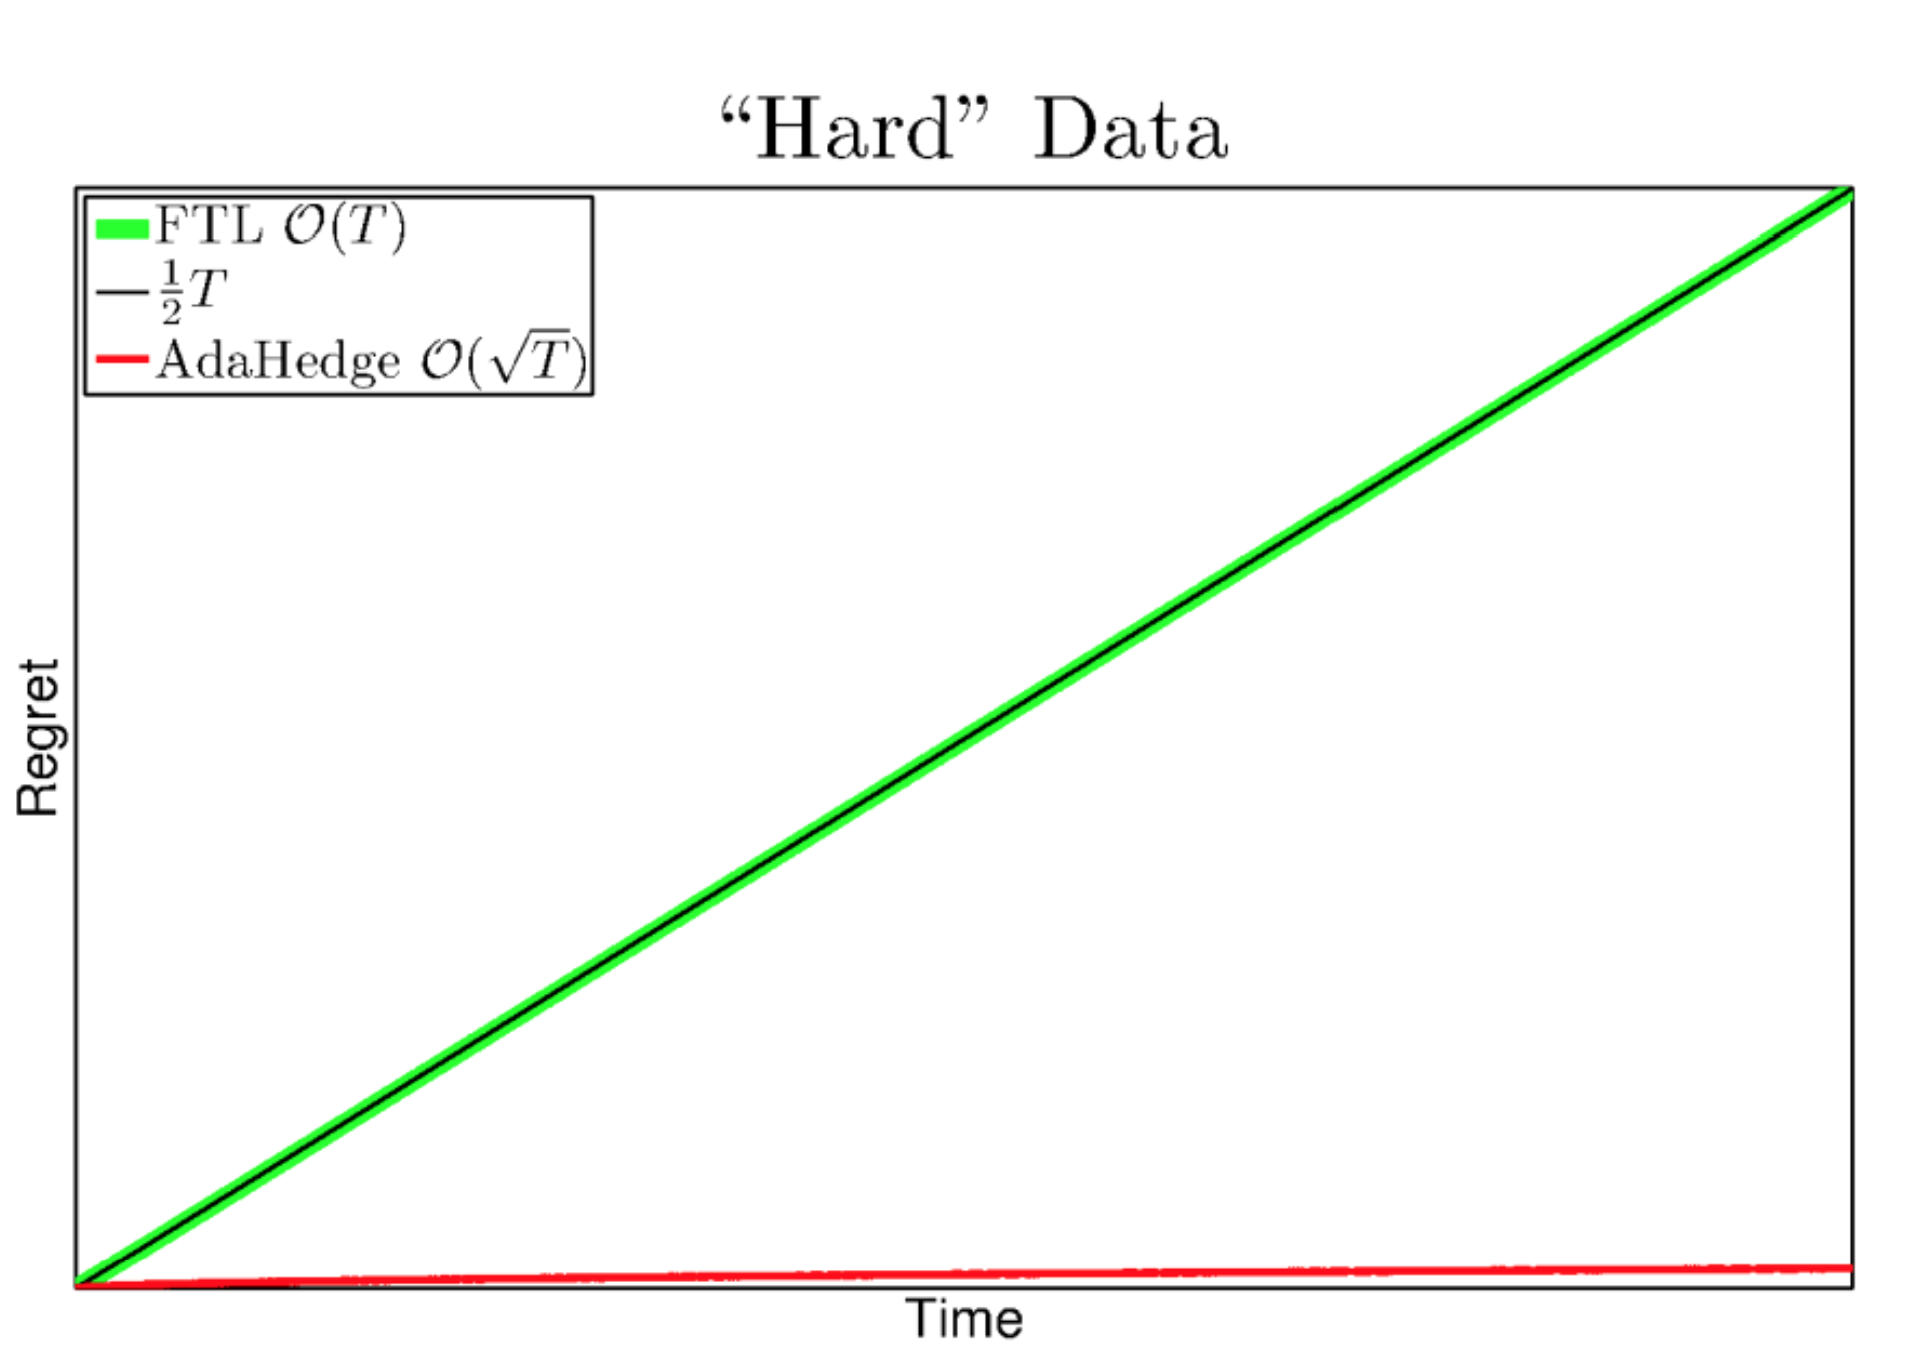
\includegraphics[width=0.9\textwidth]{figures/FTL-hard}
\end{center}
\end{minipage}
\begin{minipage}{0.1\textwidth}\end{minipage}
\pause
\begin{minipage}{0.45\textwidth}
\begin{center}
\small
extremly good \\
$\left[\begin{array}{cccccc} 0 & 0 & 1 & 0 & 1 & \ldots \\ 1 & 1 & 0 & 1 & 0 & \ldots\end{array}\right]$ 
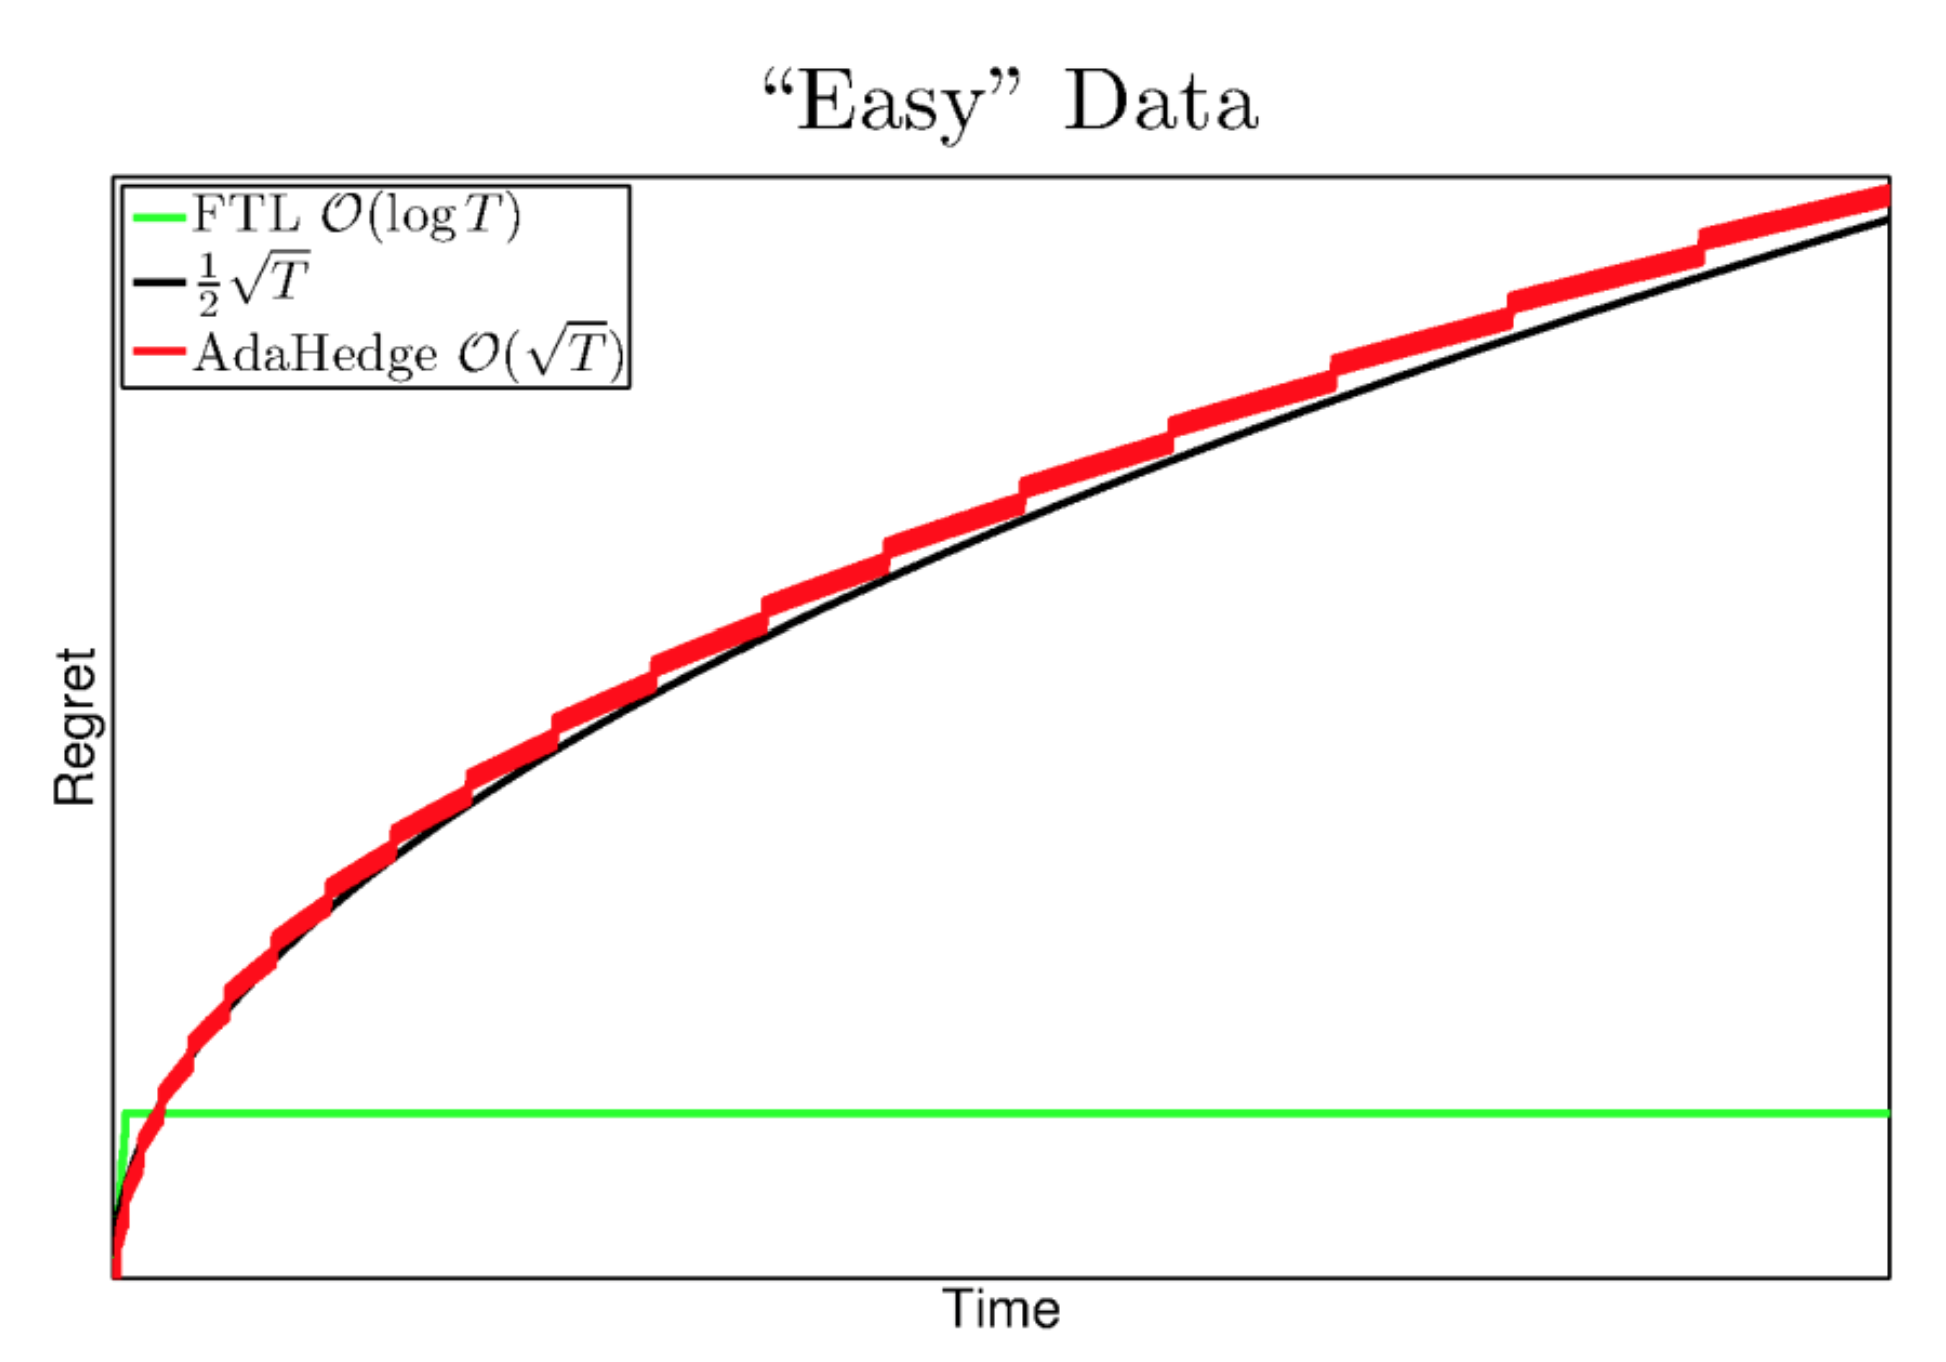
\includegraphics[width=0.9\textwidth]{figures/FTL-easy} \\
\end{center}
\end{minipage}
\scalebox{0.5}{\tiny Courtesy of Gergely Neu}
\vspace{-5cm}
\pause
\begin{center}
\begin{minipage}{0.6\textwidth}
\begin{alertblock}{}{ \bigskip \centering \Huge When is FTL good? \bigskip}\end{alertblock}
\end{minipage}
\end{center}
\vspace{3cm}

\end{frame}

\begin{frame}{FTL and the Support Function}
Support function of $\cW$:
\qquad $
\Phi(\Theta) = \max_{w\in\cW} \ip{w, \Theta}
$
\medskip

Average negative loss:
\qquad \quad$\displaystyle
\Theta_t = -\frac1t \sum_{i=1}^t f_i
$

\medskip
\pause
\begin{block}{FTL}
If $\Phi$ is differentiable at $\Theta_{t-1}$, $w_t=\nabla \Phi(\Theta_{t-1})$.
\end{block}

\medskip
\pause
\begin{alertblock}{Regret of FTL: }
\[
R_n = \sum_{t=1}^n t\,\ip{ w_{t+1}-w_t,\Theta_t} = \sum_{t=1}^{n} t\,D_{\Phi}(\Theta_t,\Theta_{t-1})
\]
{\tiny Bregman divergence: $D_{\Phi}(\theta', \theta) = \Phi(\theta') - \Phi(\theta) - \ip{ \nabla\Phi(\theta), \theta' - \theta}$}
\end{alertblock}

\begin{itemize}
\item[]
\begin{itemize}
\item Shows implicit connection with curvature...
\end{itemize}
\end{itemize}
\end{frame}


\begin{frame}{Curvature}
\footnotesize
\begin{itemize}
\item $\cW$ is $C^2$: the boundary $\bd(\cW)$ is a twice continuously differentiable submanifold of $\R^d$.
\item Gauss map: $u_{\cW} : \bd(\cW) \to \bS^{d-1}$  {\tiny(unit sphere)}
\begin{itemize}
\item continuously differentiable normal unit vector field
\end{itemize}
\item Principal curvatures: eigenvalues of  $\nabla u_{\cW}(p)$  
\begin{itemize}
\item eigenvalues of $\nabla^2 f(0)$ in the transformed coordinate system
\bigskip
\begin{center}
\hspace{-1cm}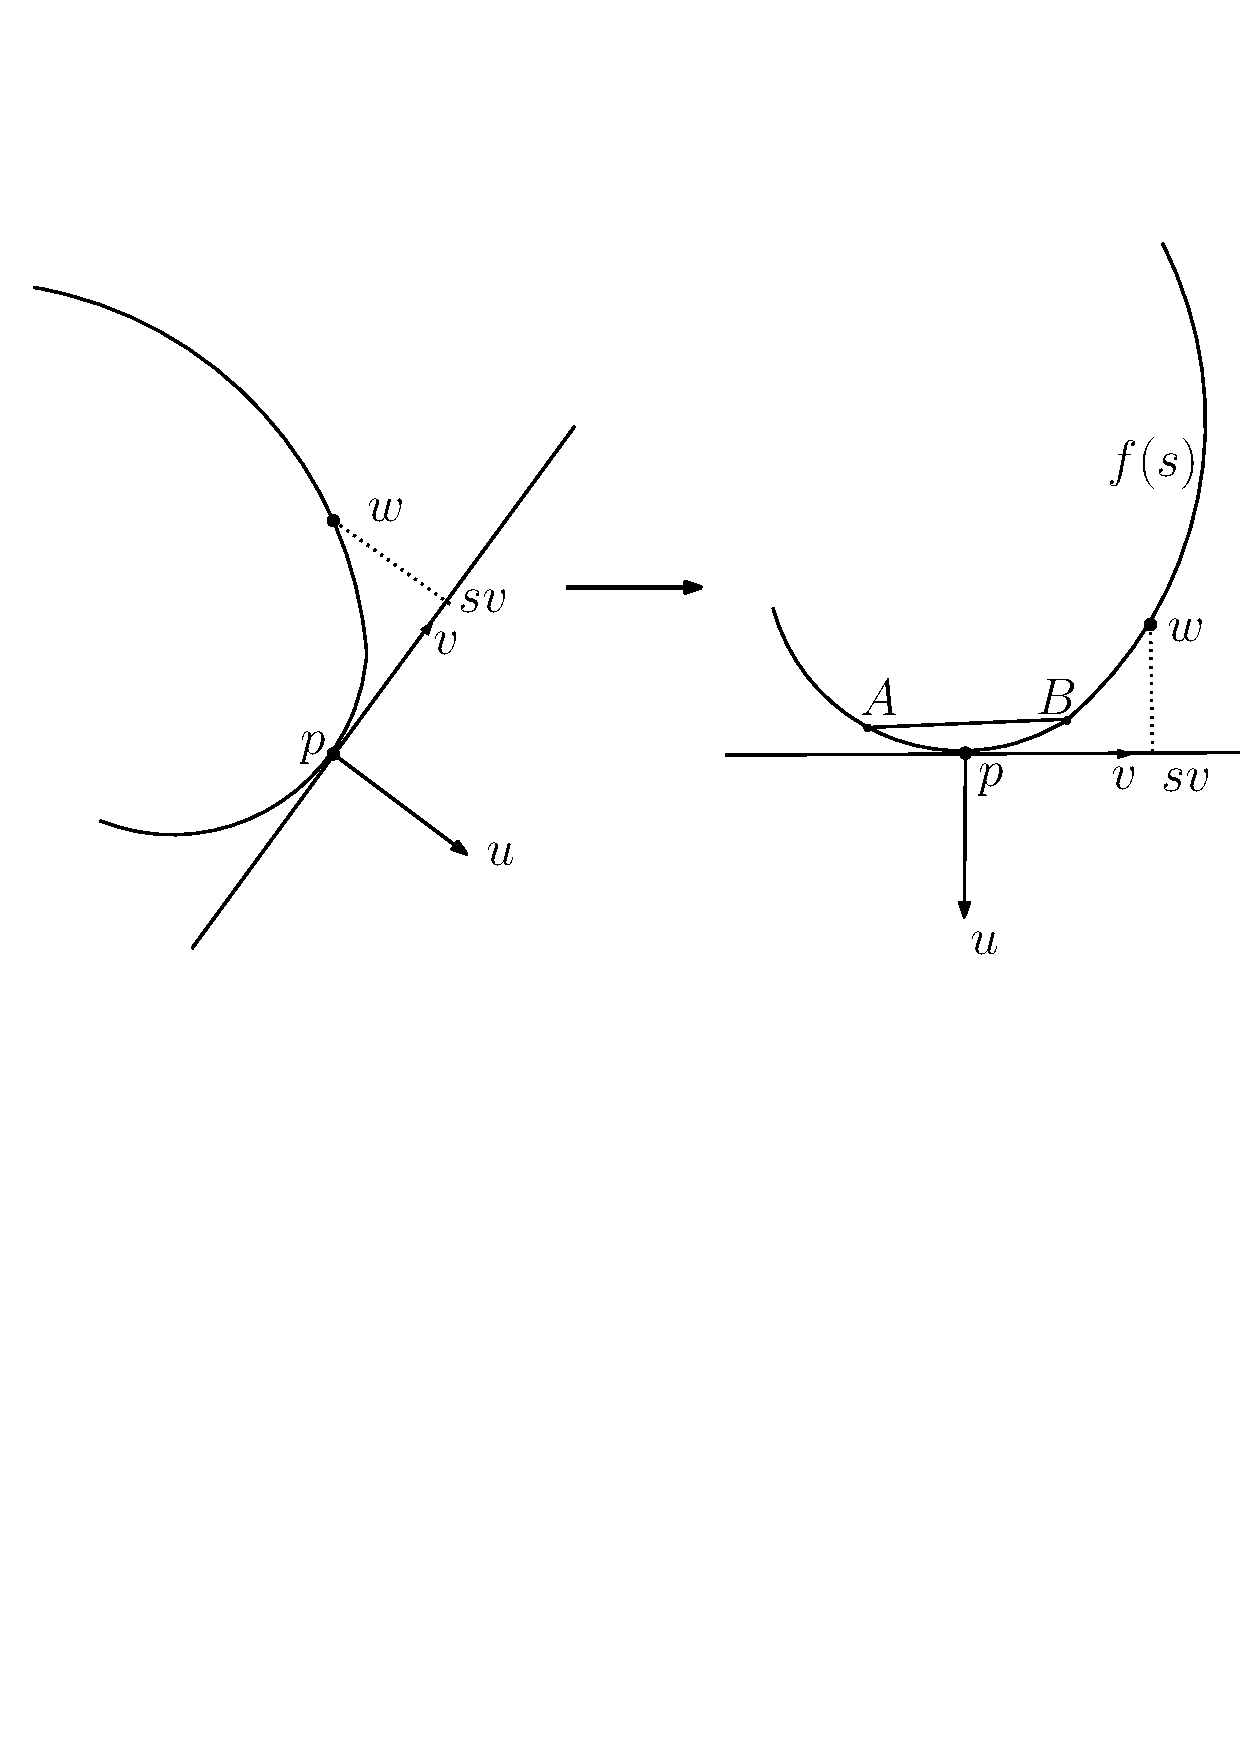
\includegraphics[width=0.55\textwidth]{figures/stronglyconvexset}
\end{center}
\smallskip
\item Example: principal curvatures of a sphere with radius $r$ are $1/r$.
\end{itemize}
\end{itemize}
\end{frame}

\begin{frame}{Examples}
The smallest principal curvature of some common convex bodies are as follows:
\begin{itemize}[<+->]\setlength{\itemsep}{10pt}
\item The smallest principal curvature $\lambda_0$ of the Euclidean ball $\cW = \set{w}{\|w\|_2\le r}$ of radius $r$ 
satisfies $\lambda_0=\frac{1}{r}$.
\item Let $Q$ be a positive definite matrix.
If $\cW = \set{w}{w^\top Q w\le 1 }$ then $\lambda_0=\lambda_{\min}/\sqrt{\lambda_{\max}}$, 
where $\lambda_{\min}$ and $\lambda_{\max}$ are the minimal, respectively, maximal eigenvalues of $Q$.
\item
In general, let $\phi:\R^d \to \R$ be a $C^2$ convex function.
Then, for $\cW = \set{w}{\phi(w)\le 1}$, 
$\lambda_0=\min_{w\in\bd(\cW)}\min_{v\,:\,\|v\|_2=1, v\perp \phi'(w) }\frac{v^{\top}\nabla^2\phi(w) v}{\|\phi'(w)\|_2}$~.
\end{itemize}
\end{frame}


\begin{frame}{Regret bound for FTL}
Assume
\begin{itemize}
\item $\cW\subset \R^d$ be a $C^2$ convex body (non-empty, compact) with $d \ge 2$;
\item the principal curvatures of the surface $\bd(\cW)$ are all at least $\lambda_0$ \\
\begin{itemize}
\item \small i.e., $\cW$ is $\lambda_0$-strongly convex;
\end{itemize}
\item $\Phi$ is differentiable at $(\Theta_t)_{t}$;
\item $M = \max_{f\in \cF} \norm{f}_2$
\item  $L_n:=\min_{1\le t \le n} \|\Theta_t\|_2 >0$. 
%\item $w_1\in \bd(\cW)$.
\end{itemize}
\begin{block}{}
Then
\[
R_n \le \frac{2M^2}{\lambda_0 L_n}(1+ \log(n))\,.
\]
\end{block}
\end{frame}

\if0
\begin{frame}{Strongly convex sets}
$\cW$ is $\lambda$-strongly convex with respect to the norm $\norm{\cdot}$ if, for  any $x,y\in \cW$ and $\gamma\in [0,1]$, the $\norm{\cdot}$-ball with origin $\gamma x + (1-\gamma) y$ and radius $\gamma(1-\gamma) \lambda \norm{x-y}^2/2 $ is included in $ \cW$. 

\bigskip

\pause

\begin{block}{Equivalence}
$\cW$ is $\lambda$-strongly convex with respect to $\norm{\cdot}_2$ if and only if the principal curvatures of the surface $\bd{\cW}$ are all at least $\lambda$.
\end{block}
\end{frame}

\begin{frame}{Strongly convex constraint sets}
Results in convex optimization:

\bigskip

\begin{itemize}
\item Exponential rates are attainable for strongly convex constraint sets if the norm of the gradients of the objective function admit a uniform lower bound. \citep{LePo66}
\bigskip
\item $O(1/n^2)$ optimization error bound (with problem-dependent constants) for the Frank-Wolfe algorithm for strongly convex and smooth objectives. \citep{garber2014faster}
\end{itemize}
\bigskip
\bigskip
\bigskip
\bigskip

\end{frame}
\fi

\begin{frame}{Regret lower bound}
Assume
\begin{itemize}
\item  $\lambda_0,L \in (0,1)$
\item $\seto{(-L,1), (-L,-1)} \subset \cF$ 
\item $\cW = \seto{(x,y):  \frac{x^2}{\lambda_0^2} + y^2 \le 1}$
\begin{itemize}
\item ellipsoid with minimal principal curvature $\lambda_0$.
\end{itemize}
\end{itemize}
\begin{block}{}
For any learning strategy, there exists a sequence of losses $f_1,f_2,\ldots \in \cF$ such that 
\[
R_n = \Omega\left(\frac{1}{L \lambda_0} \log(n)\right)
\]
and $\|\Theta_t\|_2 \ge L$ for all $t$.
\end{block}
\end{frame}

\begin{frame}{Intuition}
\begin{minipage}{0.55\textwidth}
\begin{itemize}
\item $\cW = \set{w}{\|w\|_2\le 1}$.
\item $f_t$ are i.i.d. with $\|f_t\|_\infty\le M$ and $\Exp{f_t} = \mu = (-1,0)$.
\item $w^* = (1,0)$, and thus $\inpro{w^*}{\mu} = -1$.
\item $E = \set{-\theta}{\|\theta - \mu\|_2 \le \epsilon}$, expect $-\mu_t \in E$ w.h.p. for $\epsilon=O(1/\sqrt{t})$.
\item Excess loss for $\mu_t$ is $| \tilde{B}D| \le |BD| \le  \epsilon^2 = O(1/t)$.
\item Overall regret: $O(\log(t))$
\end{itemize}
\end{minipage}\hspace{0.07\textwidth}
\begin{minipage}{0.35\textwidth}
\begin{center}
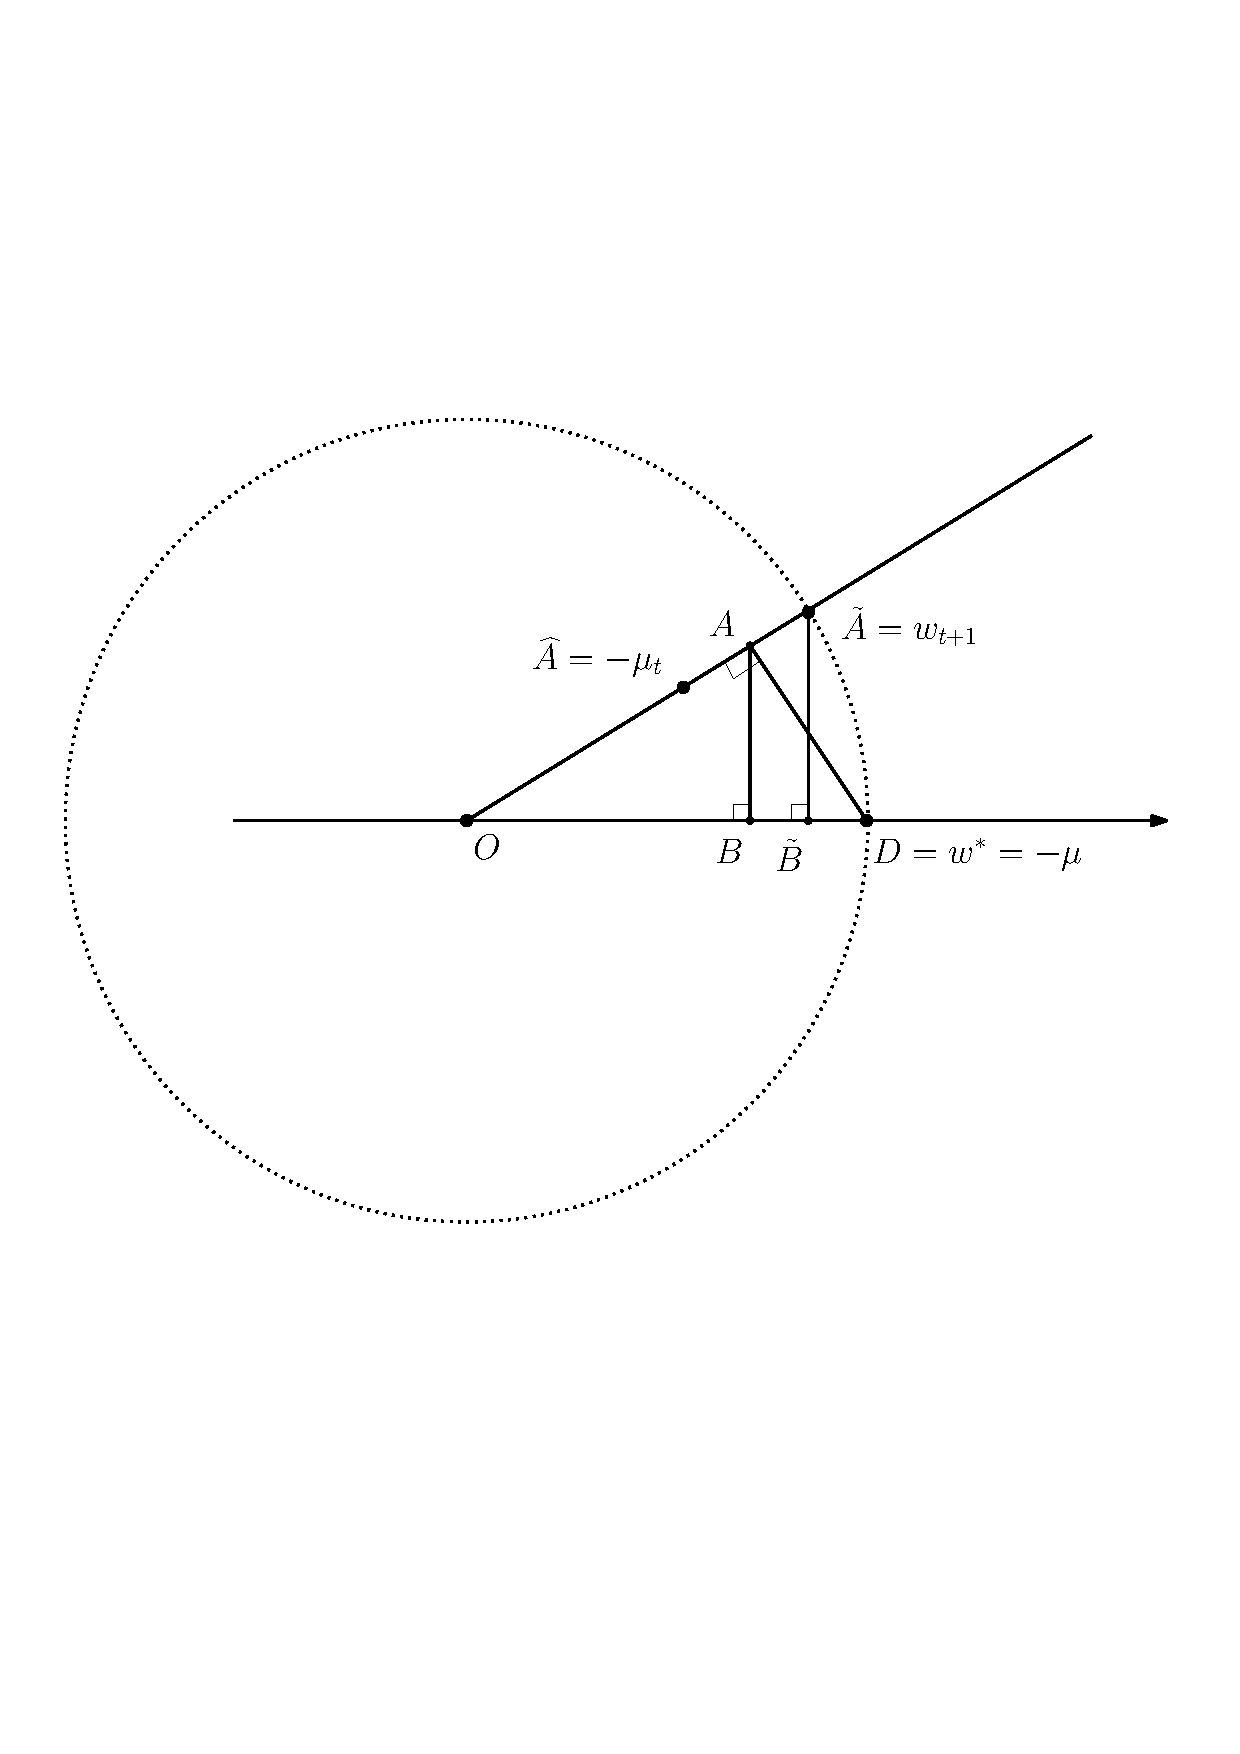
\includegraphics[width = \textwidth,
	trim={6.2cm 1cm 1.8cm 0},clip]
	{figures/ExcessError}
\end{center}
\end{minipage}
\end{frame}

\begin{frame}{Proof of the lower bound}
\begin{minipage}{0.55\textwidth}
\begin{itemize}
\item $\cW =  \seto{(x,y):  \frac{x^2}{\lambda_0^2} + y^2 \le 1}$.
\item $f_t=(-L, 2 Y_t -1)$ where $Y_t \sim$ Bernoulli($p$).
\item Beta prior on $p$ $\Rightarrow$ estimation error is $\Theta(1/\sqrt{t})$
\item Compute the regret of the Bayes optimal strategy
\end{itemize}
\end{minipage}\hspace{0.07\textwidth}
\begin{minipage}{0.35\textwidth}
\begin{center}
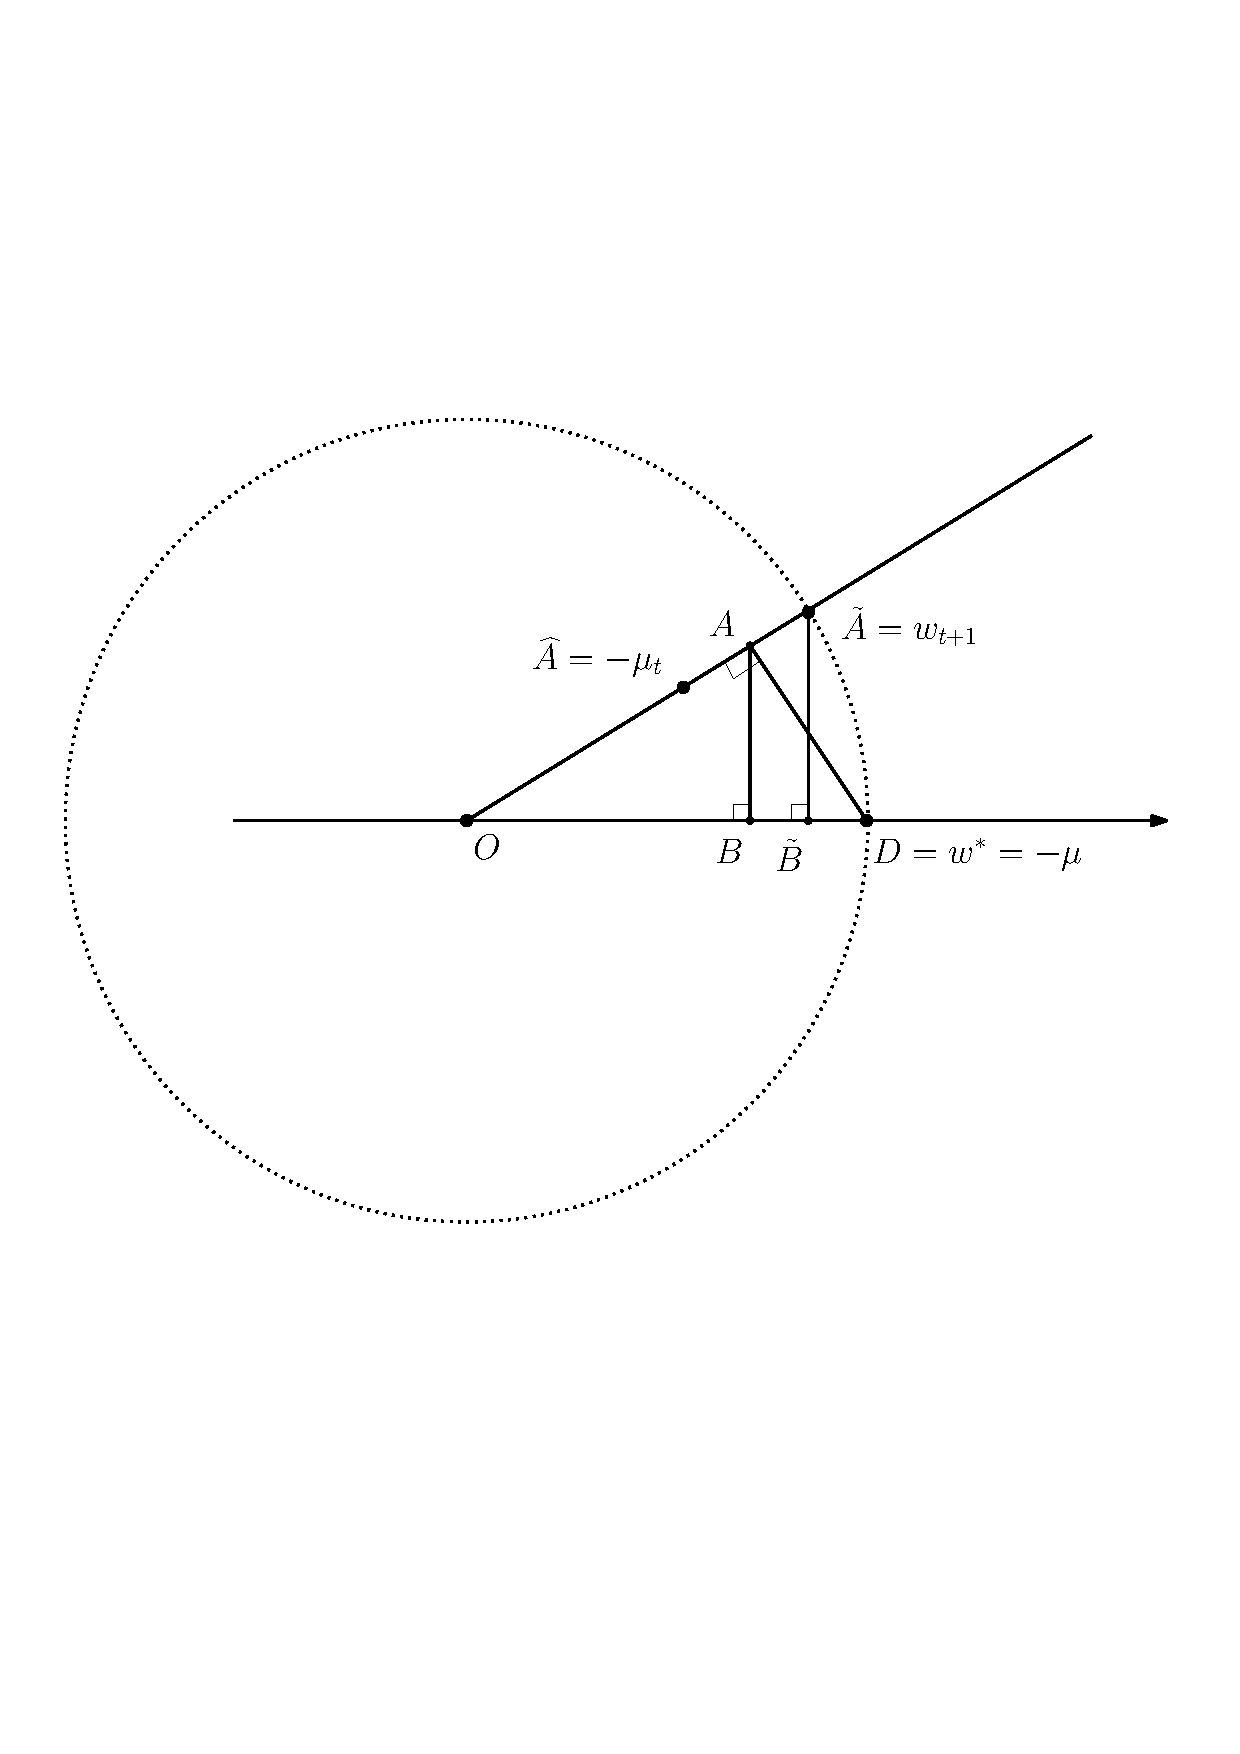
\includegraphics[width = \textwidth,
	trim={6.2cm 1cm 1.8cm 0},clip]
	{figures/ExcessError}
\end{center}
\end{minipage}
\end{frame}



\begin{frame}{Proof sketch of the upper bound}
Recall
\[
R_n = \sum_{t=1}^n t\,\ip{ w_{t+1}-w_t,\Theta_t}.
\]
\pause
We will show:
\[
\ip{ w_{t+1}-w_t,\Theta_t} \le \frac{\|\Theta_t - \Theta_{t-1}\|_2^2}{2\lambda_0 \|\Theta_{t-1}\|_2}.
\]
\pause
Also, for $M = \sup_{f\in\cF} \|f\|_2$,
$\|\Theta_{t}-\Theta_{t-1}\|_2 \le \frac{2}{t} M.$
\pause

\bigskip
Then
\begin{align*}
R_n &= \sum_{t=1}^{n} t\ip{ w_{t+1}-w_t,\Theta_t} %\\ & 
\le \sum_{t=1}^{n} \frac{t}{2\lambda_0} \frac{\|\Theta_t - \Theta_{t-1}\|_2^2}{\|\Theta_{t-1}\|_2} \\
&\le \frac{2M^2}{\lambda_0}\sum_{t=1}^{n} \frac{1}{t\|\Theta_{t-1}\|_2} \le \frac{2M^2}{\lambda_0L_n} \sum_{t=1}^{n} \frac{1}{t}
\le \frac{2M^2}{\lambda_0L_n} (1+\log(n))\,.
\end{align*}
\end{frame}


\begin{frame}{Proof sketch of the upper bound}
\begin{minipage}{0.57\textwidth}
\small
\begin{align*}
w^{(i)} &= \argmax_{w\in\cW}\inpro{w}{\theta_i} \\
\ttheta_i &= \theta_i/\|\theta_i\|_2 \\
\text{$u_\gamma(s)$:} & \quad \text{projection of outer unit}\\[-0.5em] &\text{normal vector $u_{\cW}(w)$ to $P$}\\
\gamma(0)&=w^{(1)}, \qquad u_\gamma(0)=\ttheta_1 \\
\gamma(l)&=w^{(2)}, \qquad u_\gamma(l)=\htheta_2
\end{align*}
\end{minipage}\hspace{0.03\textwidth}
\begin{minipage}{0.37\textwidth}
\begin{center}
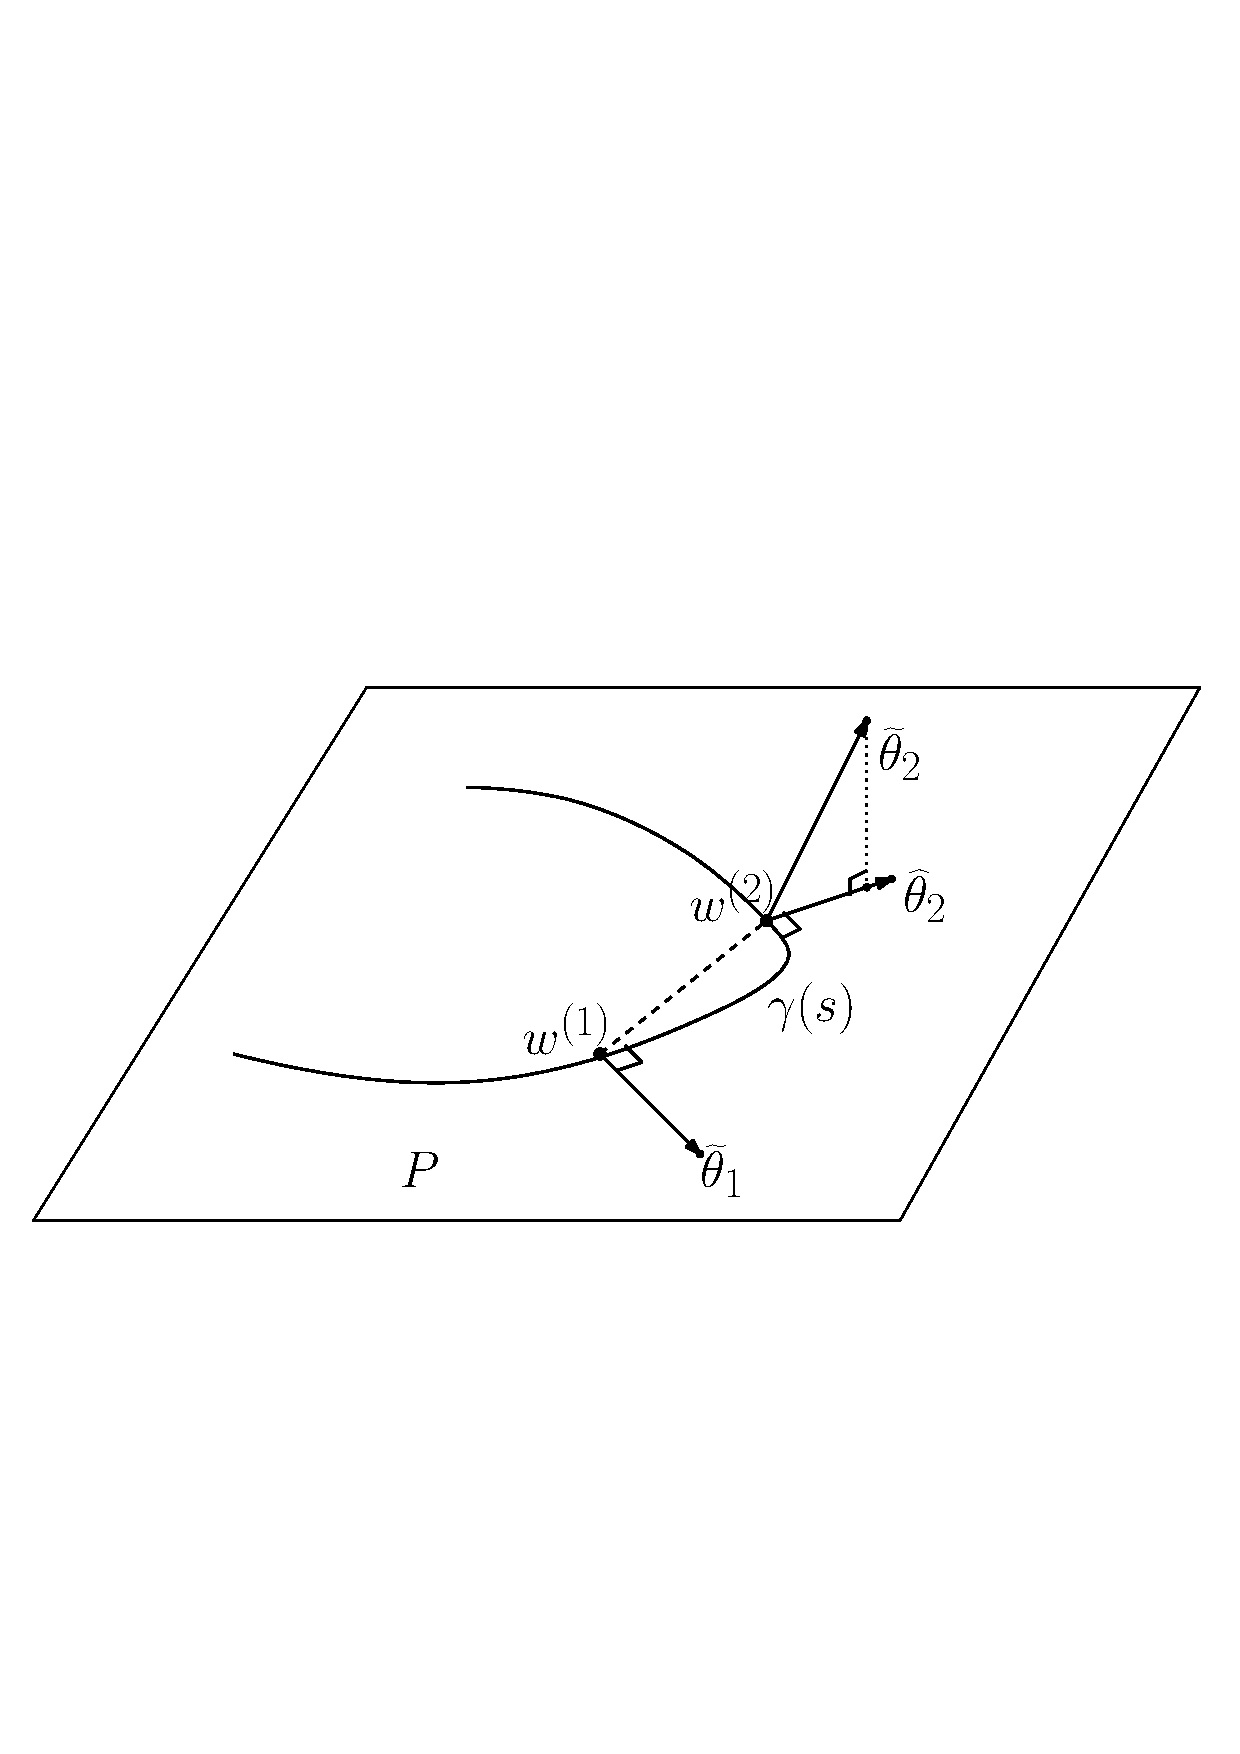
\includegraphics[width=\textwidth, trim={4.8cm 1cm 3cm 0},clip]{figures/GaussmapPro}\end{center}
\end{minipage}
\vspace{-0.2cm}
\pause
\begin{itemize}
\item Curvature: $\|u'_\gamma(s)\|_2= \lambda(s) \ge \lambda_0$ and $\gamma'(s)=\frac{u'_\gamma(s)}{\|u'_\gamma(s)\|_2}$.
\item $\gamma$ can be selected so that $\ip{\gamma'(s),\ttheta_1} \le 0$. %$\Rightarrow$ $|u_\gamma'(s)\|_2 \inpro{\gamma'(s)}{\ttheta_1} \le \lambda_0 \inpro{\gamma'(s)}{\ttheta_1}$
\end{itemize}
%\vspace{-0.2cm}
\pause
\begin{align*}
%\cos \inangle{\ttheta_1}{\ttheta_2} & \le 
\cos \inangle{\ttheta_1}{\htheta_2} &= 1 \! + \inpro{\htheta_2 - \ttheta_1}{\ttheta_1}  
= 1\!+ \!\int_{0}^{l} \inpro{u_\gamma'(s)}{\ttheta_1} \,\text{d}s  \\[0.3em]
&  \le 1 + \lambda_0 \int_0^l \ip{\gamma'(s),\ttheta_1}
 \le 1 - \lambda_0 \inpro{w^{(1)}  - w^{(2)}}{\ttheta_1}
\end{align*}
 

\end{frame}

\begin{frame}{Proof sketch of the upper bound}
From previous slide:
\[
\inpro{w^{(1)}  - w^{(2)}}{\ttheta_1} \le \frac{1-\cos \inangle{\ttheta_1}{\htheta_2}}{\lambda_0} \le \frac{1-\cos \inangle{\ttheta_1}{\ttheta_2}}{\lambda_0}~.
\]

\pause

Easy to show for any $\theta_1,\theta_2 \in \R^d$ that
\[
1- \cos \inangle{\theta_1}{\theta_2} \le \frac{1}{2} \frac{\|\theta_1 - \theta_2\|_2^2}{\|\theta_1\|_2\|\theta_2\|_2}~.
\]

\pause

Combining the above gives
\[
\inpro{w^{(1)}  - w^{(2)}}{\ttheta_1} \le \frac{1}{2 \lambda_0} \frac{\|\theta_1 - \theta_2\|_2^2}{\|\theta_1\|_2\|\theta_2\|_2}~.
\]
\end{frame}

\begin{frame}{Polytope constraint sets}
%Assume
\begin{itemize}
\item $\cW$ is a polytope
\item $W = \sup_{w_1,w_2\in \cW} \norm{w_1-w_2}_1 \qquad \text{and} \qquad
%\item $
F = \sup_{f_1,f_2\in \cF} \norm{f_1-f_2}$
\end{itemize}

\begin{block}{}
\centering \[R_n \le FW\, \sum_{t=1}^{n} \ind(w_{t+1}\neq w_{t}).\]
\end{block}

\pause

\begin{itemize}
\item $(f_t)_{1\le t \le n}$ is an i.i.d. with $\Exp{f_i} = \mu$ and $\|f_i\|_\infty \le M$. 
\item For all $\nu \in B(\mu,r)$, $\Phi$ is differentiable at $\mu$ and $\alpha \nu$ and $\beta \mu$ belong to the same face of $\cW$.
\end{itemize}
\begin{block}{}	
$$\Exp{R_n} \le 2MW \, (1+4d M^2/r^2 )\,.$$
\end{block}
\end{frame}

\begin{frame}{Adaptive algorithm}
Run ($\cA$, $\cB$)-prod of \citet{sani2014exploiting}, where algorithm
 $\cA$ is chosen to be FTRL with an appropriate regularization term, 
 while $\cB$ is chosen to be FTL. 
 
 \begin{block}{}
Then the regret of the resulting hybrid algorithm $\cH$ enjoys the following guarantees:
%(i) If FTL achieves constant regret as in the setting of \cref{cor:stocPolyhedron}, then the regret of $\cH$ is also constant.
%(ii) If FTL achieves a regret of $O(\log n)$ as in the setting of \cref{thm:R_curvesurface}, then the regret of $\cH$ is also $O(\log n)$.
%(iii) Otherwise, the regret of $\cH$ is at most $O(\sqrt{n\log n})$.
\begin{itemize}\setlength{\itemsep}{0pt}
\item If FTL achieves constant regret as in the stochastic case above, then the regret of $\cH$ is also constant.
\item If FTL achieves a regret of $O(\log n)$ as in the setting of when $\bd(\cW)$ has positive minimum curvature and $\|\Theta_t\|_2>L$, then the regret of $\cH$ is also $O(\log n)$.
\item Otherwise, the regret of $\cH$ is at most $O(\sqrt{n\log n})$.
\end{itemize}
\end{block}
\end{frame}

\begin{frame}{A direct approach}
\begin{itemize}
\item $\cW$ is the unit ball in $\R^d$.
\item $\|f_t\|_2 \le 1$ for all $t$, $F_t=\sum_{s=1}^t f_t$.
\end{itemize}

\pause
\begin{block}{Adaptive algorithm}
For $t=1,2,\ldots,n$:
\begin{itemize}
\item FTL: $\tw_t= \argmin_{w \in \cW} \ip{w,F_{t-1}}$;
\item Shrinkage: $w_t = \sigma_t \tw_t$ with 
$
\sigma_t=\begin{cases}
\frac{\|F_{t-1}\|_2}{\sqrt{\|F_{t-1}\|_2+ t+2}}& \text{if $t<n$}\\ 
\frac{\|F_{n-1}\|_2}{\sqrt{\|F_{n-1}\|_2+ n}}& \text{if $t=n$}
\end{cases}.
$
\end{itemize}
\end{block}

\pause
\begin{alertblock}{Regret bounds}
\begin{itemize}
\item If $\|\Theta_t\|_2=\|F_t/t\|_2 \ge L>0$ for all $t$, then $R_n = O(\log(n)/L)$.
\item Else $R_n=O(\sqrt{n})$. 
\end{itemize}
\end{alertblock}

\end{frame}


\begin{frame}{Proof Sketch}
Idea from \citet{abernethy2008optimal}:
\begin{align*}
	V_n & = \max_{f_1, \ldots, f_n} \sum_{t=1}^{n}\inpro{w_t}{f_t}- \min_{w\in\cW} \inpro{w}{F_n} \\
	& \le \max_{f_1,\ldots, f_{n-1}} \sum_{t=1}^{n-1}\inpro{w_t}{f_t} + \sqrt{\|F_{n-1}\|_2^2 + n} \\
	& \le \max_{f_1,\ldots, f_{n-2}} \sum_{t=1}^{n-2}\inpro{w_t}{f_t}  + \sqrt{\|F_{n-2}\|_2^2 + n-1} + \frac{1}{\sqrt{n}} \\
& \le \ldots \\
& \le \sum_{t=1}^{n}\frac{1}{\sqrt{t}} = O(\sqrt{n}).
\end{align*}
Worst case choice of $f_t$ (to maximize the bound) is orthogonal to $F_{t-1}$.
\end{frame}

\begin{frame}{Proof Sketch}
If $\|\Theta_t\| \ge L$:
\begin{align*}
	V_n & = \max_{f_1, \ldots, f_n} \sum_{t=1}^{n}\inpro{w_t}{f_t}- \min_{w\in\cW} \inpro{w}{F_n} \\
	& \le \max_{f_1,\ldots, f_{n-1}} \sum_{t=1}^{n-1}\inpro{w_t}{f_t} + \sqrt{\|F_{n-1}\|_2^2 + n} \\
	& \le \max_{f_1,\ldots, f_{n-2}} \sum_{t=1}^{n-2}\inpro{w_t}{f_t}  + \sqrt{\|F_{n-2}\|_2^2 + n-1} + \frac{1}{(n-1)L} \\
& \le \ldots \\
& \le 1+\sum_{t=1}^{n-1}\frac{1}{tL} = O(\log{n}/L).
\end{align*}
	
\end{frame}


\begin{frame}{Experiments: Stochastic data}
	\centering
	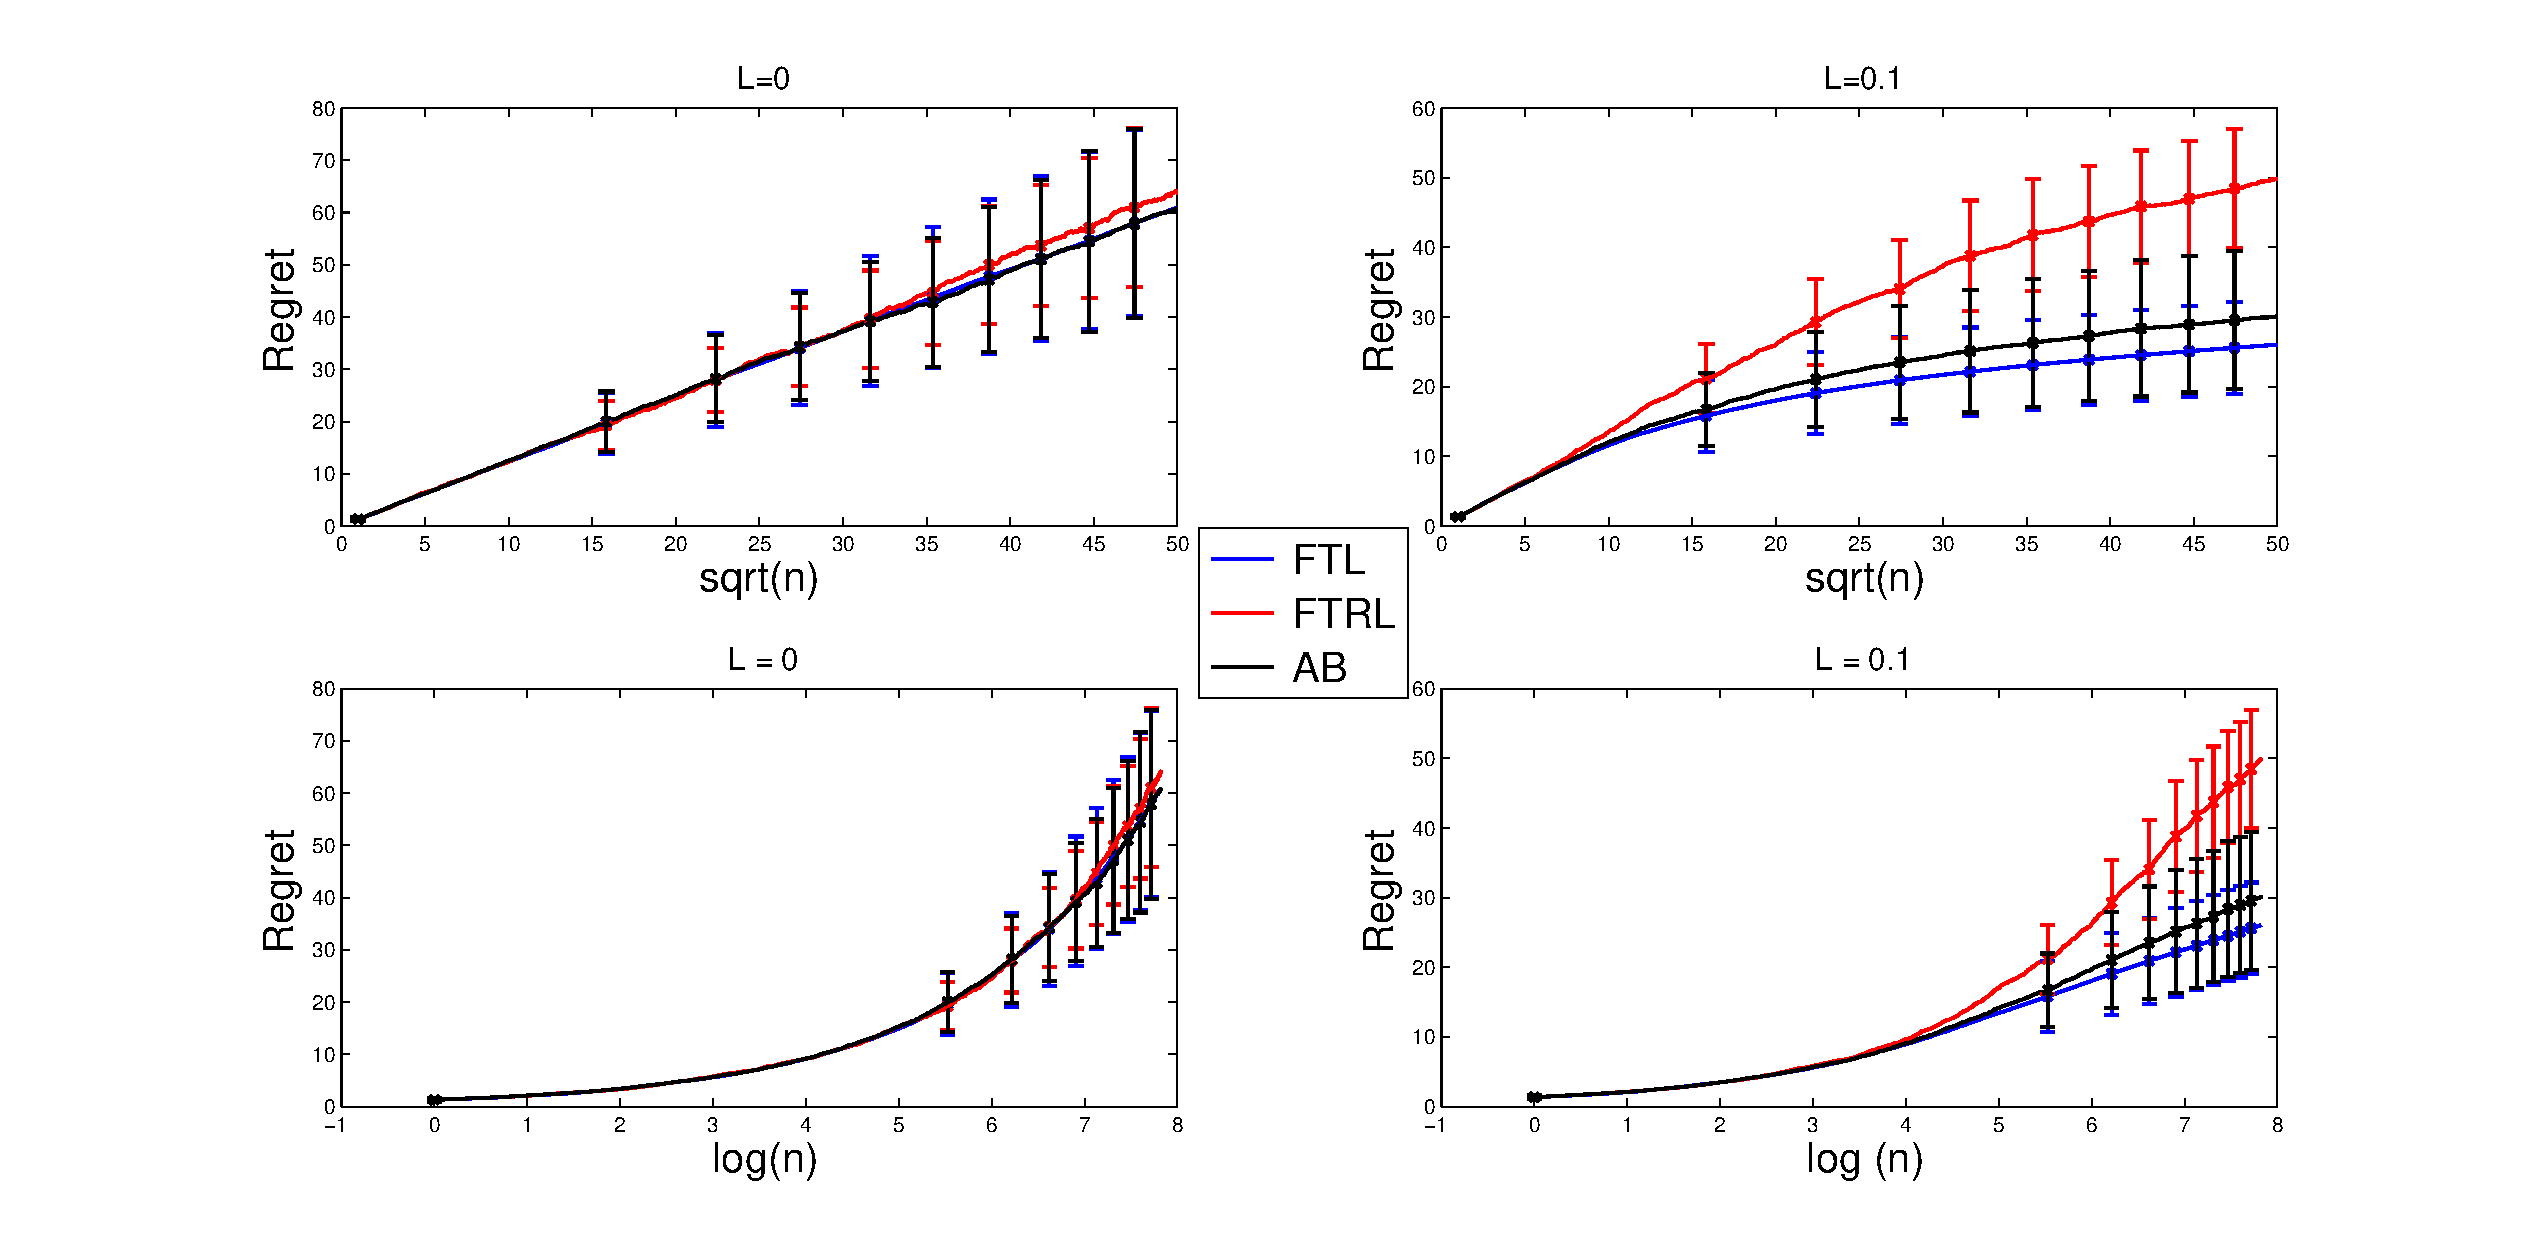
\includegraphics[height = 6cm]{figures/ExpResults/Stoc}
	
\footnotesize
\begin{itemize}
\item $\cW$: 4-dimensional ellipsoid centered at the origin
\item $f_t=L e_1 + \hf_t$ with $\hf_t$ uniformly distributed unit vector
\end{itemize}

\end{frame}

\begin{frame}{Experiments: "Half adversarial" data}
	\centering
	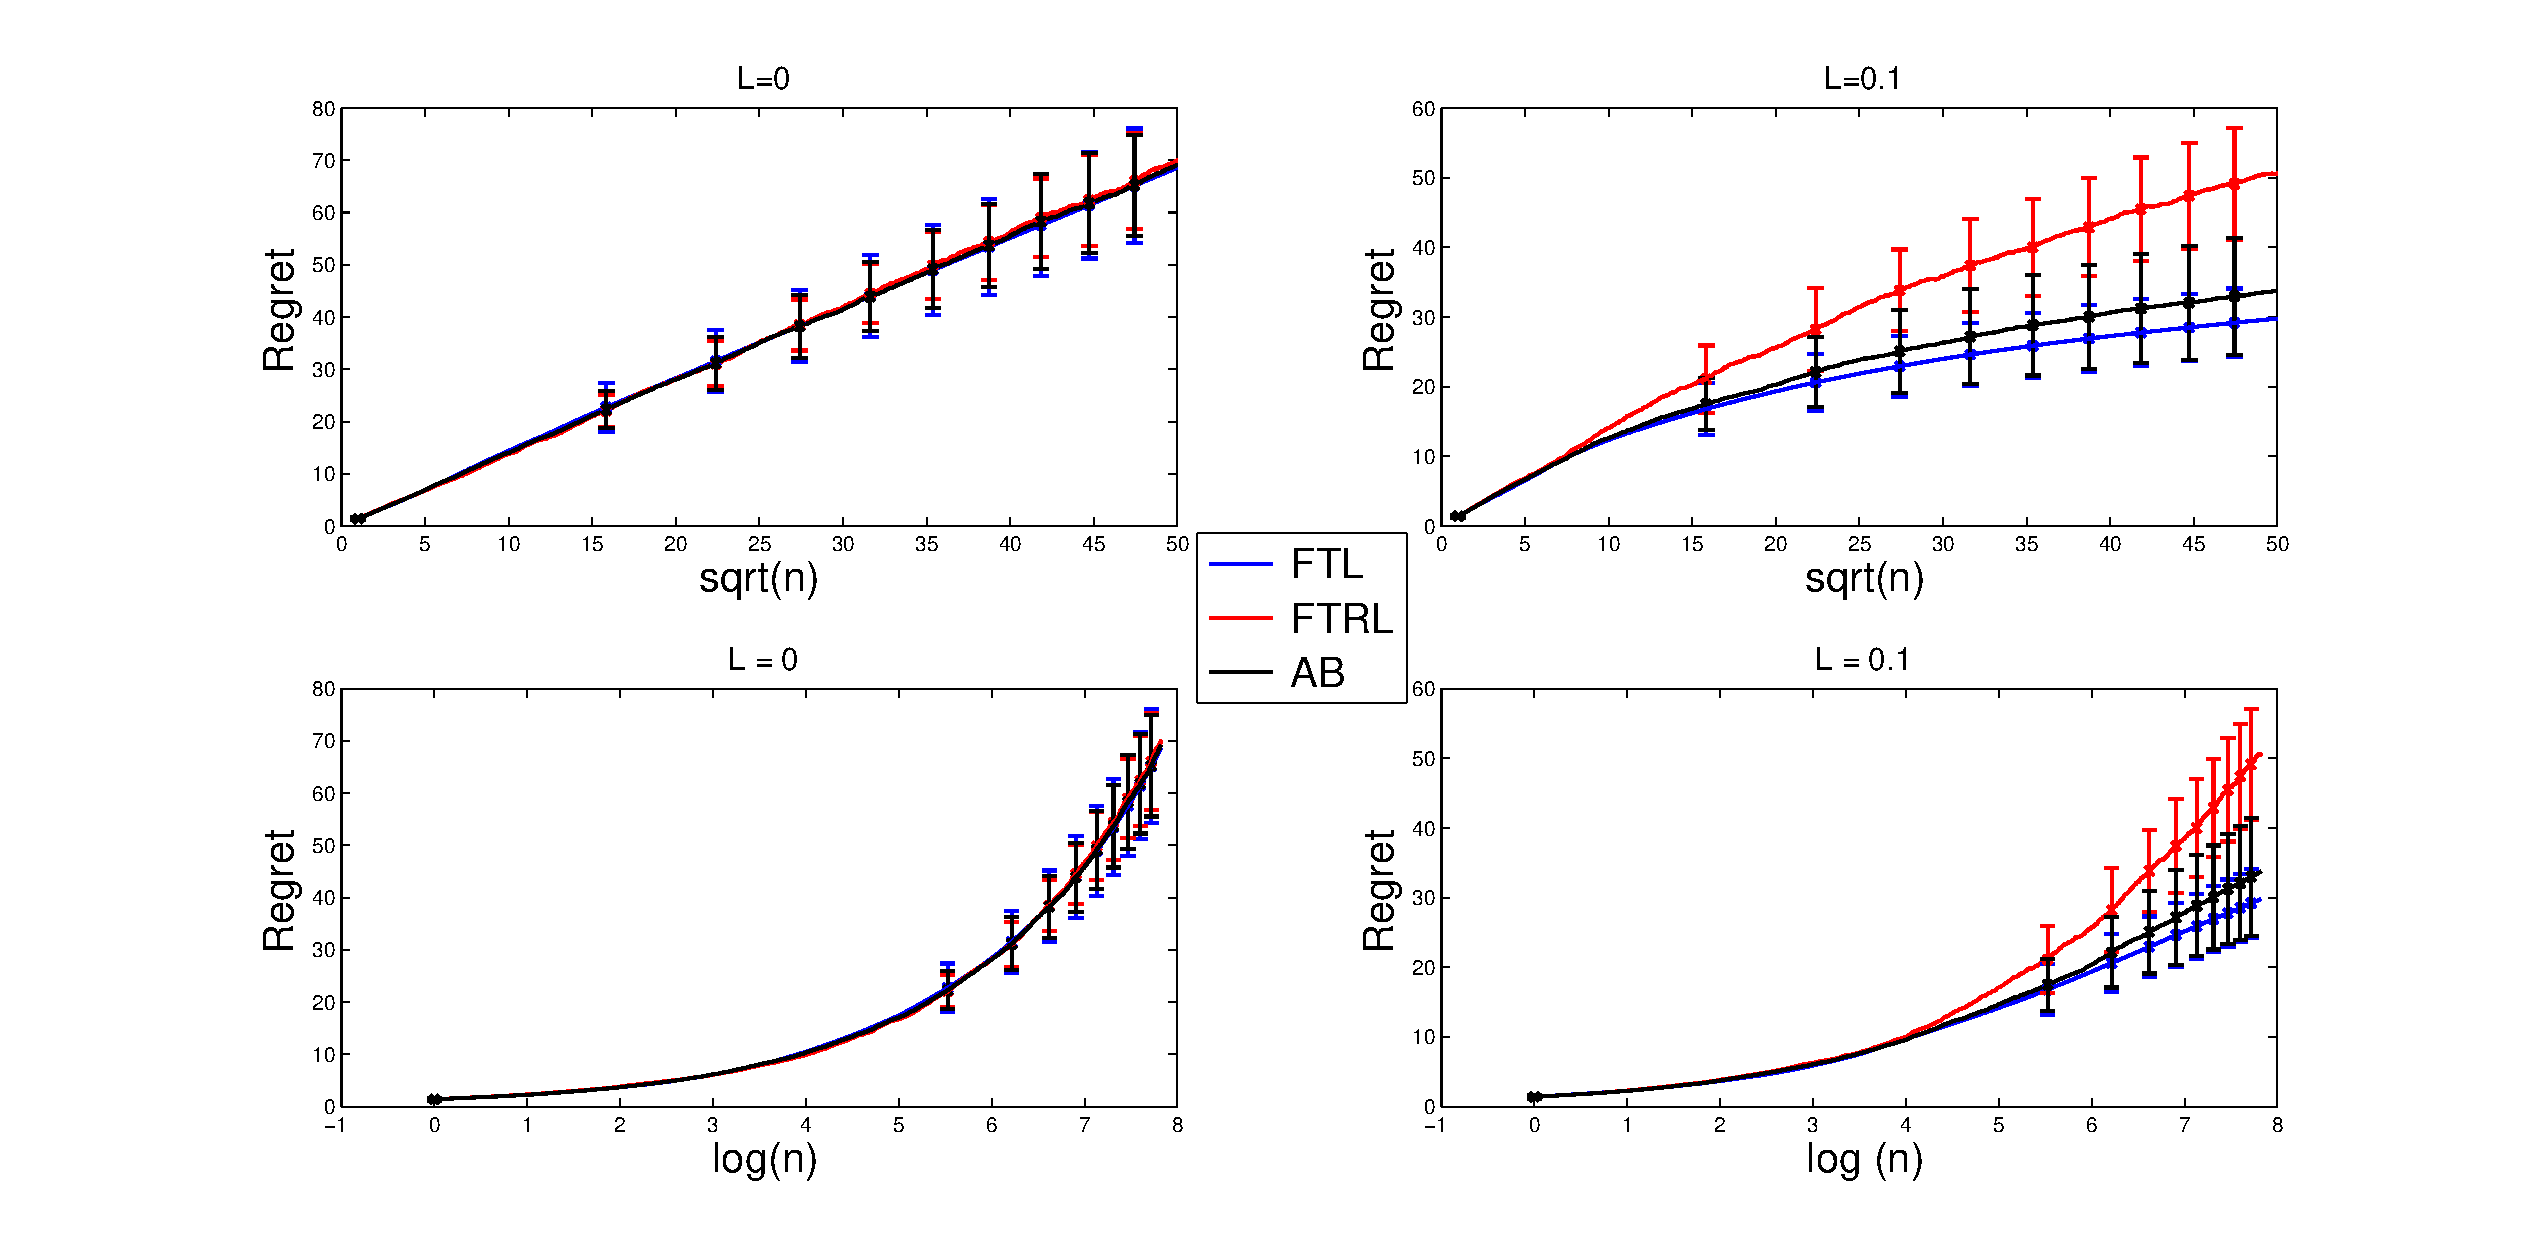
\includegraphics[height = 6cm]{figures/ExpResults/Adve}

\footnotesize
\begin{itemize}
\item $\hf_t$: $(d-1)$-dimensional unit vectors, orthogonal to $\sum_{i=1}^{t-1} \hf_i$, uniform distribution
\item $f_t=(L, \sqrt{1-L^2} \hf_t)$
\end{itemize}
\end{frame}

\begin{frame}{Experiments: Adversarial data}
	\centering
	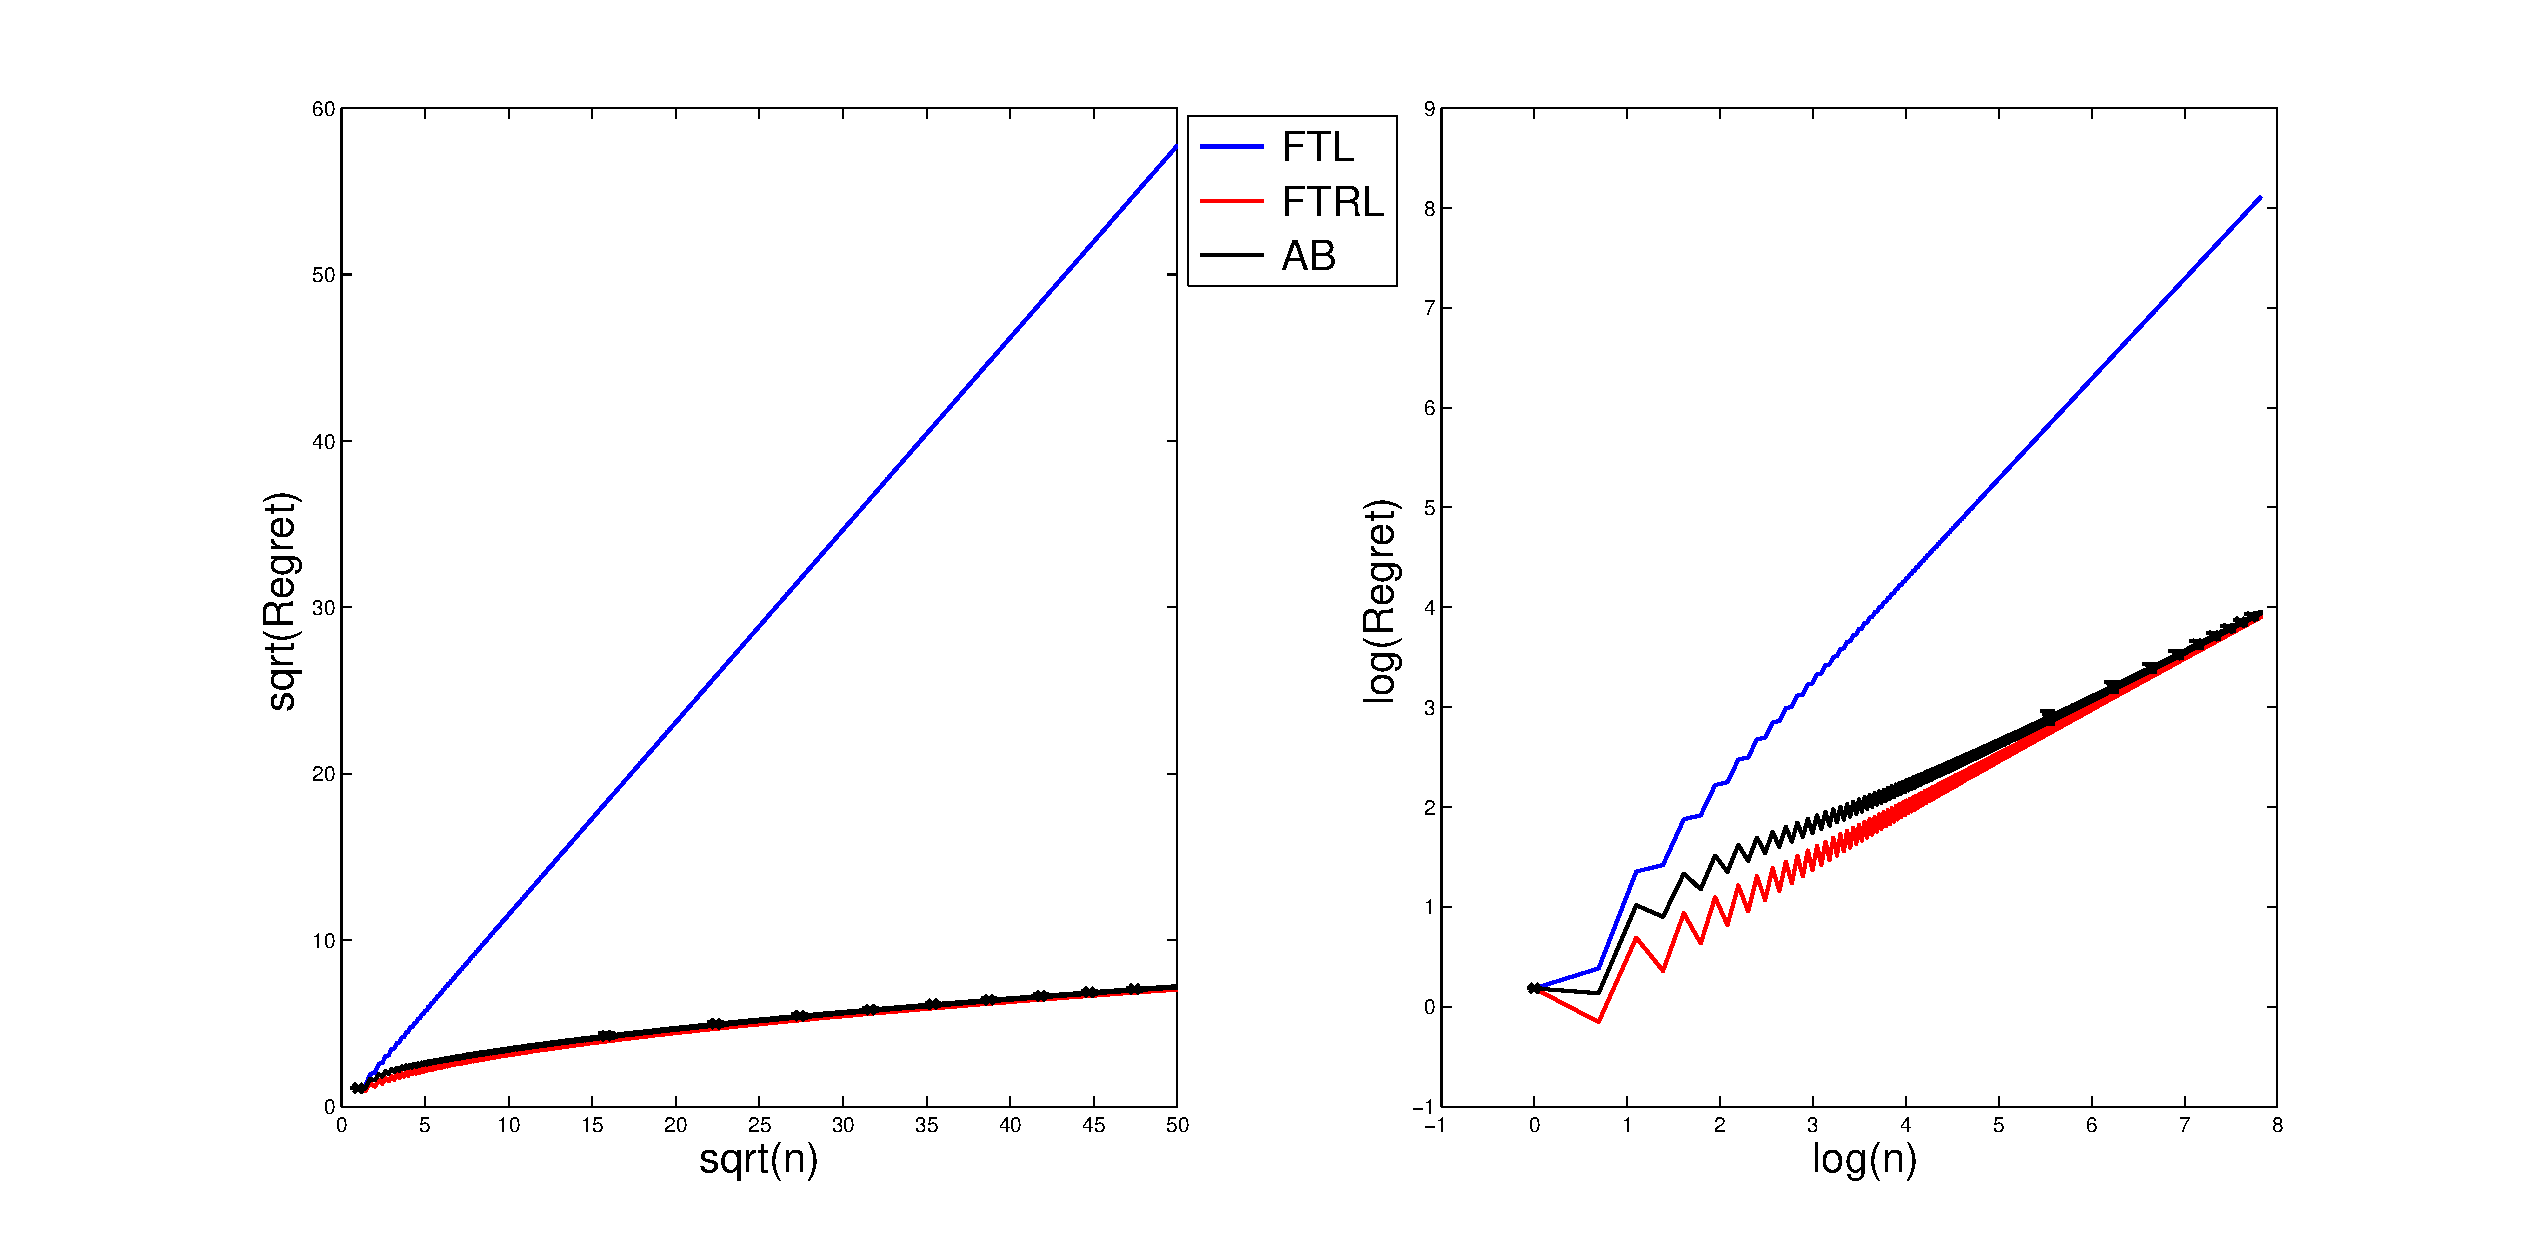
\includegraphics[height = 6cm]{figures/ExpResults/WorstCase}
\footnotesize
\begin{itemize}
\item $f_t=(\hf_t,0,\ldots,0)$
\item $(\hf_t)_t = 0.9, -1,1,-1,1,\ldots$
\end{itemize}
\end{frame}



\begin{frame}{Conclusion}
\begin{itemize}
\item Shape of the constraint set may help \bigskip
\item Other algorithms? \bigskip
\item Generalization:  \bigskip
\begin{itemize}
\item Cheating algorithm: predict $w_{t+1}$ at time $t$ \medskip
\item Control $\ell_t(w_t)-\ell_t(w_{t-1})$ \medskip
\item What else can help? \medskip
\item Conjecture: $\ell_t$ $\alpha$-expconcave, minimum curvature $\lambda_0$ $\Rightarrow$ $O(\log(n)/(\alpha+\lambda_0))$ regret
\end{itemize}
\end{itemize}
\end{frame}

%%%%%%%%%%%%%%%%%%%%%%%%%%%%%%%%%%%%%%%%
\section*{References}
%%%%%%%%%%%%%%%%%%%%%%%%%%%%%%%%%%%%%%%%

%\begin{frame}[allowframebreaks]{References}
\begin{frame}{References}
    \Fontvi
%	\scriptsize 
	\begin{multicols}{2} % from \usepackage{multicol}
	\bibliography{reference}
	\bibliographystyle{plainnat}
	\end{multicols}
\end{frame}
%%%%%%%%%%%%%%%%%%%%%%%%%%%%%%%%%%%%%%%%


% All of the following is optional and typically not needed. 
%\appendix
%\section<presentation>*{\appendixname}
%\subsection<presentation>*{For Further Reading}
%
%\begin{frame}[allowframebreaks]
%  \frametitle<presentation>{For Further Reading}
%    
%  \begin{thebibliography}{10}
%    
%  \beamertemplatebookbibitems
%  % Start with overview books.
%
%  \bibitem{Author1990}
%    A.~Author.
%    \newblock {\em Handbook of Everything}.
%    \newblock Some Press, 1990.
% 
%    
%  \beamertemplatearticlebibitems
%  % Followed by interesting articles. Keep the list short. 
%
%  \bibitem{Someone2000}
%    S.~Someone.
%    \newblock On this and that.
%    \newblock {\em Journal of This and That}, 2(1):50--100,
%    2000.
%  \end{thebibliography}
%\end{frame}
%



\end{document}




